%%------------------------------------------------------
%% Conversion of Ford and Coulston to LaTEX
%%------------------------------------------------------

%%------------------------------------------------------
%% Document formatting standards.
%% references labels		figure:<camelCase>
%%						table:<camelCase>
%%						section:<dash seperated>
%%------------------------------------------------------


\documentclass[11pt]{book}
\usepackage{graphicx}
\usepackage{imakeidx}			% Enables Index functionality
\usepackage{hyperref}			% Enable hyperlinks to email and URLs

%% Lots of packages needed for tables
\usepackage{xcolor,colortbl}	% Enable colors in tables
\usepackage{multirow}
\usepackage{longtable}		%Enables multiplage tables
\newcommand{\ul}{\underline}
\definecolor{Gray}{gray}{0.85}


\makeindex

\begin{document}

\frontmatter
\title{{\Huge Design for Electrical and Computer Engineers} \\
				Theory, Concepts, and Practice}
\author{Ralph M. Ford and Christopher S. Coulston}
\date{}
\maketitle


This document was prepared with \LaTeX.
\\
\\
\\

Copyright \copyright  2024 by Christopher Coulston
\\
\\

All rights reserved.  No part of this publication may be reproduced, 
stored in a retrieval system, or transmitted, in any form or by any
means, electronic, mechanical, photocopying, recording, or otherwise
without prior written permission of the author.

\section{About the Authors}\label{about-the-authors}


\includegraphics[width=1in,height=1.39583in]{./Fig/image1.jpeg}Ralph
Ford obtained his Ph.D. and M.S. degrees in Electrical Engineering from
the University of Arizona in 1994 and 1989 respectively. He obtained his
B.S. in Electrical Engineering from Clarkson University in 1987. He
worked for the IBM Microelectronics Division in East Fishkill, NY from
1989-1991, where he developed machine vision systems to inspect
electronic packaging modules for mainframe computers. Ralph also has
experience working for IBM Data Systems and the Brookhaven National
Laboratory. He joined the faculty at Penn State Erie, The Behrend
College in 1994. Ralph has experience teaching electronics and software
design, as well as teaching the capstone design course sequence in the
electrical, computer, and software engineering programs. His research
interests are in engineering design, image processing, machine vision,
and signal processing. Ralph is currently Director of the School of
Engineering at Penn State Behrend. He also serves as a program evaluator
for ABET. He was awarded a Fulbright Scholarship to study at the Brno
University of Technology in the Czech Republic in 2005.

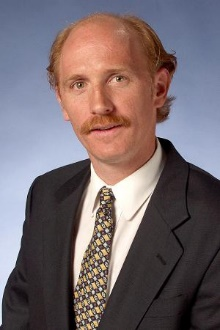
\includegraphics[width=1in,height=1.5in]{./Fig/image2.jpeg}Chris
Coulston obtained his Ph.D. in Computer Science and Engineering from the
Pennsylvania State University in 1999. He obtained his M.S. and B.S in
Computer Engineering from the Pennsylvania State University in 1994 and
1992 respectively. Chris has industry experience working for IBM in
Manassas, VA and Accu-Weather in State College, PA. He joined the
faculty at Penn State Erie, The Behrend College in 1999. He has
experience teaching design-oriented courses in digital systems, embedded
systems, computer architecture, and database management systems. Chris'
research interests are in Steiner tree routing algorithms and artificial
life. He is currently an Associate Professor of Electrical and Computer
at Penn State Behrend and also serves as Chairperson of the program.


\tableofcontents
\section{Preface}\label{preface}

This book is written for undergraduate students and teachers engaged in
electrical and computer engineering (ECE) design projects, primarily in
the senior year. The objective of the text is to provide a treatment of
the design process in ECE with a sound academic basis that is integrated
with practical application. This combination is necessary in design
projects because students are expected to apply their theoretical
knowledge to bring useful systems to reality. This topical integration
is reflected in the subtitle of the book: Theory, Concepts, and
Practice. Fundamental theories are developed whenever possible, such as
in the chapters on functional design decomposition, system behavior, and
design for reliability. Many aspects of the design process are based
upon time-tested concepts that represent the generalization of
successful practices and experience. These concepts are embodied in
processes presented in the book, for example, in the chapters on needs
identification and requirements development. Regardless of the topic,
the goal is to apply the material to practical problems and design
projects. Overall, we believe that this text is unique in providing a
comprehensive design treatment for ECE, something that is sorely missing
in the field. We hope that it will fill an important need as capstone
design projects continue to grow in importance in engineering education.

We have found that there are three important pieces to completing a
successful design project. The first is an understanding of the design
process, the second is an understanding of how to apply technical design
tools, and the third is successful application of professional skills.
Design teams that effectively synthesize all three tend to be far more
successful than those that don't. The book is organized into three parts
that support each of these areas.

The first part of the book, the \emph{Design Process}, embodies the
steps required to take an idea from concept to successful design. At
first, many students consider the design process to be obvious. Yet it
is clear that failure to understand and follow a structured design
process often leads to problems in development, if not outright failure.
The design process is a theme that is woven throughout the text;
however, its main emphasis is placed in the first four chapters. Chapter
1 is an introduction to design processes in different ECE application
domains. Chapter 2 provides guidance on how to select projects and
assess the needs of the customer or user. Depending upon how the design
experience is structured, both students and faculty may be faced with
the task of selecting the project concept. Further, one of the important
issues in the engineering design is to understand that systems are
developed for use by an end-user, and if not designed to properly meet
that need, they will likely fail. Chapter 3 explains how to develop the
Requirements Specification along with methods for developing and
documenting the requirements. Practical examples are provided to
illustrate these methods and techniques. Chapter 4 presents concept
generation and evaluation. A hallmark of design is that there are many
potential solutions to the problem. Designers need to creatively explore
the space of possible solutions and apply judgment to select the best
one from the competing alternatives.

The second part of the book, \emph{Design Tools}, presents important
technical tools that ECE designers often draw upon. Chapter 5 emphasizes
system engineering concepts including the well known functional
decomposition design technique and applications in a number of ECE
problem domains. Chapter 6 provides methods for describing system
behavior, such as flowcharts, state diagrams, data flow diagrams and a
brief overview of the Unified Modeling Language (UML). Chapter 7 covers
important issues in testing and provides different viewpoints on testing
throughout the development cycle. Chapter 8 addresses reliability theory
in design, and reliability at both the component and system level is
considered.

The third part of the book focuses on \emph{Professional Skills}.
Designing, building, and testing a system is a process that challenges
the best teams, and requires good communication and project management
skills. Chapter 9 provides guidance for effective teamwork. It provides
an overview of pertinent research on teaming and distills it into a set
of heuristics. Chapter 10 presents traditional elements of project
planning, such as the work breakdown structure, network diagrams, and
critical path estimation. It also addresses how to estimate manpower
needs for a design project. Chapter 11 addresses ethical considerations
in both system design and professional practice. Case studies for ECE
scenarios are examined and analyzed using the IEEE (Institute of
Electrical and Electronics Engineers) Code of Ethics as a basis. The
book concludes with Chapter 12, which contains guidance for students
preparing for oral presentations, often a part of capstone design
projects.

\textbf{Features of the Book}

This book aims to guide students and faculty through the steps necessary
for the successful execution of design projects. Some of the features
are listed below.

\begin{itemize}
\item
  Each chapter provides a brief motivation for the material in the
  chapter followed by specific learning objectives.
\item
  There are many examples throughout the book that demonstrate the
  application of the material.
\item
  Each end-of-chapter problem has a different intention. Review problems
  demonstrate comprehension of the material in the chapter. Application
  problems require the solution of problems based upon the material
  learned in the chapter. Design problems are directly applicable to
  design projects and are usually tied in with the Project Application
  section.
\item
  Nearly all chapters contain a Project Application section that
  describes how to apply the material to a design project.
\item
  Some chapters contain a Guidance section that represents the author's
  advice on application of the material to a design project.
\item
  Checklists are provided for helping students assess their work.
\item
  There are many terms used in design whose meaning needs to be
  understood. The text contains a glossary with definitions of design
  terminology. The terms defined in the glossary (Appendix A) are
  indicated by \emph{\textbf{italicized-bold}} highlighting in the text.
\item
  All chapters conclude with a Summary and Further Reading section. The
  aim of the Further Reading portion is to provide pointers for those
  who want to delve deeper into the material presented.
\item
  The book is structured to help programs demonstrate that they are
  meeting the ABET (accreditation board for engineering programs)
  accreditation criteria. It provides examples of how to address
  constraints and standards that must be considered in design projects.
  Furthermore, many of the professional skills topics, such as teamwork,
  ethics, and oral presentation ability, are directly related to the
  ABET Educational Outcomes. The requirements development methods
  presented in Chapter 3 are valuable tools for helping students perform
  on cross-functional teams where they must communicate with
  non-engineers.
\item
  An instructor's manual is available that 
  contains not only solutions, but guidance from the authors on teaching
  the material and managing student design teams. It is particularly
  important to provide advice to instructors since teaching design has
  unique challenges that are different than teaching engineering science
  oriented courses that most faculty are familiar with.
\item
  PowerPoint\textsuperscript{TM} presentations are available for
  instructors through McGraw-Hill
\item
  There are a number of complete case study student projects available
  in electronic form for download by both students and instructors and
  available at.
  These projects have been developed using the processes provided in
  this book.
\end{itemize}

\textbf{How to Use this Book}

There are several common models for teaching capstone design, and this
book has the flexibility to serve different needs. Particularly,
chapters from the Professional Skills section can be inserted as
appropriate throughout the course. Recommended usage of the book for
three different models of teaching a capstone design course is
presented.

\begin{itemize}
\item
  \textbf{Model I.} This is a two-semester course sequence. In the first
  semester, students learn about design principles and start their
  capstone projects. This is the model that we follow. In the first
  semester the material in the book is covered in its entirety. The
  order of coverage is typically Chapters 1--3, 9, 4--6, 10--11, and
  7--8. Chapter 9 (Teams and Teamwork) is covered immediately after the
  projects are identified and the teams are formed. Chapters 10 (Project
  Management) and 11 (Ethical and Legal Issues) are covered after the
  system design techniques in Chapters 5 and 6 are presented. Students
  are in a good position to create a project plan and address ethical
  issues in their designs after learning the more technical aspects of
  design. Chapter 12 (Oral Presentations) is assigned to students to
  read before their first oral presentation to the faculty. The course
  concludes with principles of testing and system reliability (Chapter 7
  and 8). We assign a good number of end-of-chapter problems and have
  quizzes throughout the semester. By the end of the first semester,
  design teams are expected to have completed development of the
  requirements, the high-level or architectural design, and developed a
  project plan. In the second semester, student teams implement and test
  their designs under the guidance of a faculty advisor.
\item
  \textbf{Model II}. This two-semester course sequence is similar to
  Model I with the difference being that the first semester is a lower
  credit course (often one credit) taught in a seminar format. In this
  model chapters can be selected to support the projects. Some of the
  core chapters for consideration are Chapters 1--5, which take the
  student from project selection to functional design, and Chapters
  9--11 on teamwork, project management, and ethical issues. Other
  chapters could be covered at the instructor's discretion. The use of
  end-of-chapter problems would be limited, but the project application
  sections and example problems in the text would be useful in guiding
  students through their projects.
\item
  \textbf{Model III}. This is a one-semester design sequence. Here, the
  book would be used to guide students through the design process.
  Chapters for consideration are 1--5 and 9--10, which provide the
  basics of design, teamwork, and project management. The project
  application sections and problems could be used as guidance for the
  project teams.
\end{itemize}

\textbf{Acknowledgements}

Undertaking this work has been a challenging experience and could not
have been done without the support of many others. First, we thank our
families for their support and patience. They have endured many hours
and late evenings that we spent researching and writing. Melanie Ford is
to be thanked for her diligent proofreading efforts. Bob Simoneau, the
former Director of the Penn State Behrend School of Engineering, has
been a great supporter of the book and has also lent his time in reading
and providing comments. Our school has a strong design culture, and this
book would not have happened without that emphasis; our faculty
colleagues need to be recognized for developing that culture. Jana
Goodrich and Rob Weissbach are two faculty members with whom we have
collaborated on other courses and projects. They have influenced our
thinking in this book, particularly in regard to project selection,
requirements development, cost estimation, and teamwork. We must also
recognize the great collaborative working environment that exists at
Penn State Behrend, which has allowed this work to flourish. Our
students have been patient in allowing us to experiment with different
material in the class and on the projects. Examples of their work are
included in the book and are greatly appreciated. John Wallberg
contributed the disk drive diagnostics case study in Chapter 11 that we
have found very useful for in-class discussions. John developed this
while he was a student at MIT. Thanks to Anne Maloney for her
copyediting of the manuscript. 

Finally, we would like to thank the external reviewers of the book for
their thorough reviews and valuable ideas. They are Frederick C. Berry
(Rose-Hulman Institute of Technology), Mike Bright (Grove City College),
Geoffrey Brooks (Florida State University Panama City Campus) Wils L.
Cooley (West Virginia University), D. J. Godfrey (US Coast Guard
Academy), and Michael Ruane (Boston University).

We hope that you find this book valuable, and that it motivates you to
create great designs. We welcome your comments and input. Please feel
free to email us.

Ralph M. Ford, \href{mailto:rmf7@psu.edu}{\nolinkurl{rmf7@psu.edu}}

Christopher S. Coulston,
 \href{mailto:coulston@mines.edu}{\nolinkurl{coulston@mines.edu}}


\mainmatter 					% Now Use Arabic numerals for page numbers


\chapter{The Engineering Design Process}
\section{The Engineering Design Process}
\graphicspath{ {./chapter01/Fig} }

\begin{itquote}
\textbf{en-gi-neer (n)} 
\textit{1. One versed in the design, construction, and
use of machines. 2. One who employs the innovative and methodical
application of scientific knowledge and technology to produce a device,
system, or process, which is intended to satisfy human needs.} ---American College Dictionary
\end{itquote}

Take a moment to read and analyze the key elements of the two
definitions presented above. If you are an engineering student or
practicing engineer, do you think that this definition applies to you?
The first definition uses the terms \emph{design} and
\emph{construction}. People like to think of themselves as designers.
Why is that so? The answer may be in the combination of the term
\emph{construction,} and from the second definition, the idea of
\emph{innovation}. Applying innovation and creativity to produce
something new is a wonderfully rewarding process. The great thing about
being an engineer is that it allows you to be a creative designer. That
is generally not the way the profession is viewed. What is the
difference between engineering design and other types of design that are
associated with creativity such as interior design, fashion design, or
webpage design? The answer is supplied in the second definition which
states \emph{''\ldots methodical application of scientific knowledge and
technology\ldots{}}'' As an engineering student, you have studied a
great deal of math, science, and fundamental technology, but probably
have had limited exposure to creative and innovative design.

The definition also contains the somewhat contradictory terms
\emph{innovative} and \emph{methodical}. If there is an established and
methodical way of employing a scientific principle or process, it does
not seem to allow much room for creativity and innovation. The truth is
that the two concepts are in competition with each other, but a good
engineer realizes this and utilizes both effectively. The definition
also indicates that engineers design to satisfy human needs, an
important, yet often overlooked point. That means that when designing
systems, it is necessary to determine the user's needs and the ethical
application of the technology.

This book aims to help electrical and computer engineers become
effective designers, to better understand professional practices, and to
provide guidance for executing design projects. This chapter presents
the processes by which designs are realized, the characteristics of
successful engineers, and an overview of the book.

\section*{Learning Objectives}
\noindent\rule{\linewidth}{1pt}
By the end of this chapter, the reader should:
\begin{itemize}
\item Understand what is meant by engineering design.
\item  Understand the phases of the engineering design process.
\item  Be familiar with the attributes of successful engineers.
\item  Understand the objectives of this book.
\end{itemize}

\section{The Engineering Design Process}

ABET (formerly known as Accreditation Board of Engineering and
Technology) provides the following definition of engineering design
{[}ABE03{]}.
\index{ABET}

\begin{quote}
Engineering design is the process of devising a system, component, or
process to meet desired needs. It is a decision-making process (often
iterative), in which the basic sciences, mathematics, and engineering
sciences are applied to convert resources optimally to meet a stated
objective. Among the fundamental elements of the design process are the
establishment of objectives and criteria, synthesis, analysis,
construction, testing, and evaluation.
\end{quote}

The definition indicates that, in engineering design, different phases
of the process have to be re-visited and the deliverables for each phase
updated as necessary. Realistic problems are complex with many potential
solutions; the goal is not to find just any solution, but the best one
given the constraints and available resources. This requires the
application of sound judgment, decision-making skills, and patience in
constantly evaluating progress towards a solution. The definition
identifies some common elements of the design process, such as
establishment of criteria, synthesis, construction, and testing.

\emph{\textbf{Design processes}} embody the steps required to take an
idea from concept to realization of the final system, and are
problem-solving methodologies that aim to develop a system that best
meets the customer's need within given constraints. This is not all that
different from some everyday processes, such as preparing dinner. Say
you are hungry and need to eat dinner before you can go to see a movie
that starts in one hour. The constraints are time, money, food, your
tastes, and nutritional value if you are health-conscious. You
brainstorm and come up with the options of making dinner at home, going
to a restaurant, or buying something to eat at the theater. Based on
these options, you then select the solution based on your evaluation of
the best one. This is similar in philosophy to the stages of design
processes where you have a problem to solve, constraints, and a number
of potential solutions to select from.

A related term is known as the \emph{product realization process}. The
product realization process is broader in scope, including aspects such
as entrepreneurship, market research, financial planning, product
pricing, and market strategy. Many technologies have their own
particular design processes that have evolved over time and have been
found by practitioners in the field to be valuable. For example,
different methodologies are applied in the design of integrated circuits
(VLSI), embedded systems, and software systems, yet they all have some
degree of commonality, such as requirements analysis, technical design,
and system test. Design processes continue to evolve. One field in which
this is particularly true is in software design due to the constantly
changing nature of software and the special challenges that large
software projects pose.

Cross {[}Cro00{]} identified two types of design
processes---prescriptive and descriptive. As the name implies,
\emph{\textbf{prescriptive design processes}} set down an exact process,
or systematic recipe, for realizing a system. Prescriptive design
processes are often algorithmic in nature and expressed using flow
charts with decision logic. An example of a prescriptive process is
shown in Figure~\ref{figure:prescriptiveDesign}, 
which describes the front end of the design process
where the problem and requirements are determined. A decision block is
included where the requirements are examined to determine if they
satisfy the needs of the problem. \emph{\textbf{Descriptive processes}}
are less formal, describing typical activities involved in realizing
designs with less emphasis on exact sequencing. The distinction between
descriptive and prescriptive processes is not always clear, however, and
some processes may be considered more strongly associated with one
property than the other. Cross makes an important point in stating that
design processes are sometimes viewed as common sense and thus ignored,
resulting in failed products. Cross cites two good reasons to adhere to
design processes: 1) they formalize thought processes to ensure good
practices are followed, leading to better and more innovative solutions,
and 2) they keep all members of the team synchronized in terms of
understanding where they are in the design process.

\begin{figure}[h]
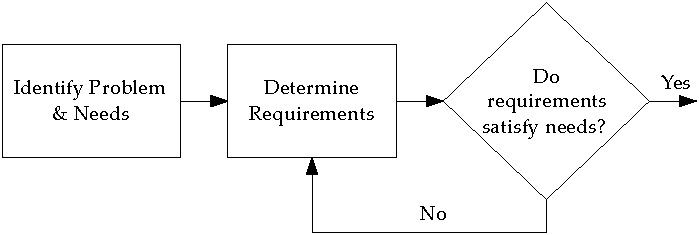
\includegraphics[width=3.8in,height=1.27in]{image1}
\caption{A prescriptive design process for problem
identification and requirements selection.}
\label{figure:prescriptiveDesign}
\end{figure}

A descriptive process that is widely applicable to design problems is
shown in Figure~\ref{figure:overviewDesignProcess}. 
In a perfect world, the process starts with the
identification of the problem, proceeds clockwise to research, followed
the requirements phase, and so on until the system or device is
delivered and goes into service (maintenance phase). This scenario is
unrealistic, ignoring the iterative nature of design where the design
team alternates between different phases as necessary. Consequently,
links are inserted that allow transitions between all the different
phases of the

\begin{figure}[h]
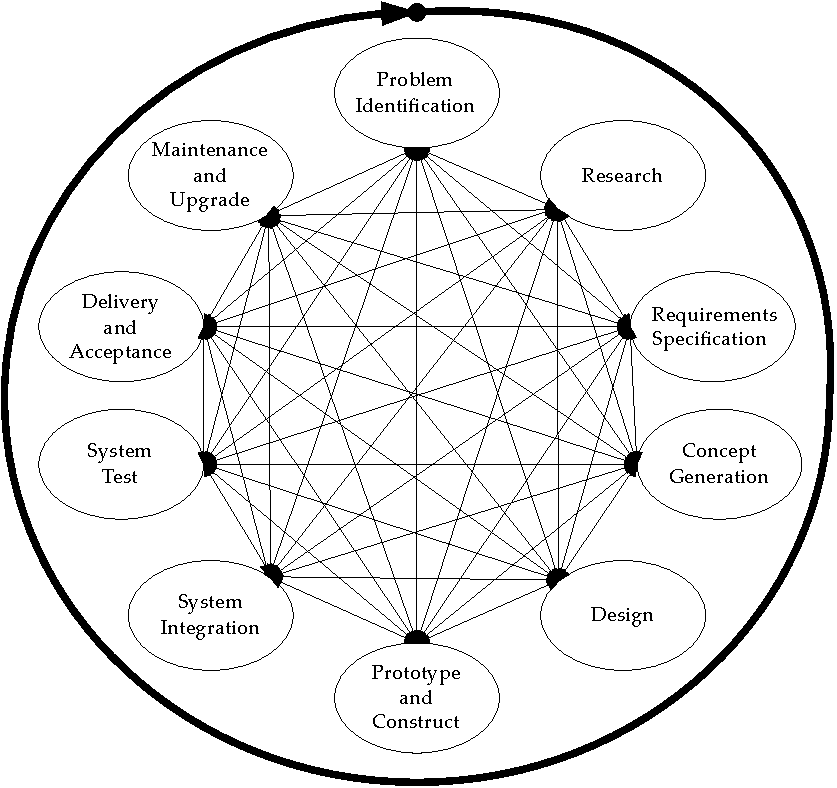
\includegraphics[width=5in,height=4.7in]{image2}
\caption{ A descriptive overview of the design process.}
\label{figure:overviewDesignProcess}
\end{figure}

design process. Of course, transitions between certain phases are
unreasonable or very costly. It is virtually impossible to move directly
from problem identification to system integration without developing a
design concept first. It is much more likely for engineers to alternate
between nearby phases in the process, such as problem identification,
research, requirements specification, and concept generation. This does
not mean that you can't move between phases that are not in close
proximity in the model. For instance, the customer's needs may change
while in the design phase, necessitating re-evaluation of the needs,
correction of the requirements specification, and system redesign---all
at a substantial cost in time and money. Studies have shown that the
cost required to correct errors or make changes increases exponentially
as the project lifetime increases, as presented in Figure~\ref{figure:costVsLife}.

\begin{figure}[h]
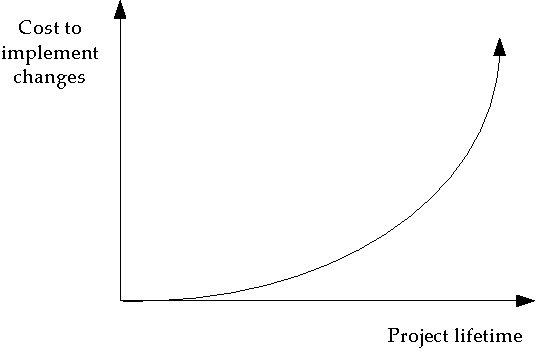
\includegraphics[width=3in,height=2in]{image3}
\caption{The cost to implement design changes increases exponentially with project lifetime.}
\label{figure:costVsLife}
\end{figure}

\subsection{Elements of the Design Process}

Nearly all the phases of the design process in Figure~\ref{figure:overviewDesignProcess} 
are covered in this book, with the exception of the maintenance phase. The objective of
the first phase, \emph{\textbf{problem identification}}, is to identify
the problem and customer needs. This occurs in a variety of ways, from
someone conceiving a new idea to a client coming to you with a problem
to solve. In either case, it is important to determine the true needs
for the product, device, or system (terms that are used interchangeably
throughout the book and often referred to as systems). Failure to
correctly identify the needs has negative ramifications for the entire
process, typically resulting in costly redesigns, or even worse,
abandonment of the project.

In the \emph{\textbf{research phase}} the design team conducts research
on the basic engineering and scientific principles, related
technologies, and existing solutions. The objective is to become experts
on the problem, save time and money by not re-inventing the wheel, and
be positioned to develop new and innovative solutions.

The \emph{\textbf{Requirements Specification}} articulates what the
system must do for it to be successful and to be accepted by the
customer. It is important to focus on what the system must do, as
opposed to how the solution will be implemented. This is challenging
since engineers tend to focus on solutions and propose implementations
early in the process. This is not surprising since engineering education
focuses on solving problems rather than specifying them. The
requirements are the mission statement that guides the entire project,
and if properly developed, provide flexibility for creativity and
innovation in developing solutions.

In \emph{\textbf{concept generation},} many possible solutions to the
problem are developed. The hallmark of design is that it is open-ended,
meaning that there are multiple solutions to the problem and the
objective is to develop the one that best meets the requirements and
satisfies the constraints. In this phase, wild creativity is encouraged,
but it is ultimately tempered with critical evaluation of the competing
alternatives.

In the \emph{\textbf{design phase},} the team iteratively develops a
technical solution, ultimately producing a detailed system design. Upon
its completion, all major systems and subsystems are identified and
described using an appropriate model that depends upon the particular
technology being employed.

In the \emph{\textbf{prototyping and construction phase},} different
elements of the system are constructed and tested. In rapid prototyping,
the objective is to model some aspect of the system, demonstrating
functionality to be employed in the final realization. Many prototypes
are discarded or modified as the system evolves---the idea is to
experiment, demonstrate proof-of-concept principles, and improve
understanding. Prototypes may be used anywhere in the process---you may
present the client with prototypes after the concept generation phase,
or they may be utilized in the design phase to test a design idea, or as
the final system is tested and developed.

During \emph{\textbf{system integration},} all of the subsystems are
brought together to produce a complete working system. This phase is
challenging and time-consuming since many different pieces of the design
must be interfaced, and the team must work closely to make it all work.
Care taken in the design phase to clearly communicate the functionality
and interfaces between subsystems aids in system integration. System
integration is closely tied to the \emph{\textbf{test phase}}, where the
overall system is tested to demonstrate that it meets the requirements.

Ultimately the system is \emph{delivered} to the customer where it is
likely that they will test it using a mutually agreed upon process.
Development does not necessarily end when the system goes into service,
as it will likely enter the \emph{\textbf{maintenance phase}} where it
is maintained, upgraded to add new functionality, or where design
problems are corrected. Following and understanding the design process
improves the probability of successful system development. The process
is flexible, and the designer needs to transition between different
phases in order to bring the system to realization. Design is an
iterative process---you may not fully understand everything necessary in
any given phase and have to revisit different steps as the system
evolves. That is not a license for not trying to develop the best design
you can on the first attempt---by all means do so---but realize that
flexibility and a willingness to change the design are necessary.

\subsection{Technology Specific Design Processes}

Different application domains have developed specialized processes for
technology-specific design. One such example is VLSI (Very Large Scale
Integration) design. A typical VLSI design process is shown in Figure~\ref{figure:VLSIdesign}
 {[}Wol02{]}. In this model the system specification is used to
develop the system architecture. The system architecture is composed of
the major functional units that constitute an integrated circuit. Each
functional unit is then designed at the gate logic level, which is
subsequently designed at the circuit (transistor) level, and finally the
circuit elements are laid out on the silicon chip. This is an excellent
demonstration of the divide-and-conquer approach to design, where a
complex system is broken down into lower levels of abstraction and each
of these is further broken down until the design objectives are met.

\begin{figure}[h]
 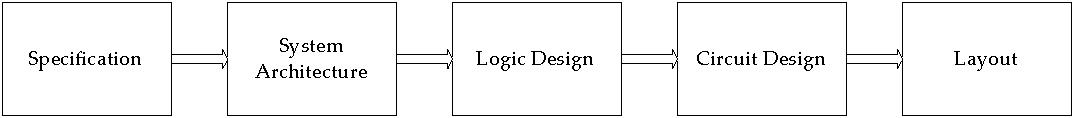
\includegraphics[width=5.5in,height=0.60417in]{image4}
\caption{A process for integrated circuit (VLSI) design {[}Wol02{]}.}
\label{figure:VLSIdesign}
\end{figure}

Next, consider the design process for embedded computer systems shown in
Figure~\ref{figure:embedded DesignProcess}. 
Embedded systems are combined hardware/software systems
embedded into a larger system to perform dedicated application specific
operations. Embedded systems are employed in automobiles, DVD players,
and digital cameras to name a few applications. Performance issues
dominate embedded applications, and the designer needs to partition
tasks between software and hardware to achieve optimum performance. This
design process is somewhat prescriptive with phases for requirements
gathering, specifications, and architectural design. The process
reflects the unique nature of embedded systems with separate software
and hardware design blocks, married together by the interface design.

\begin{figure}[h]
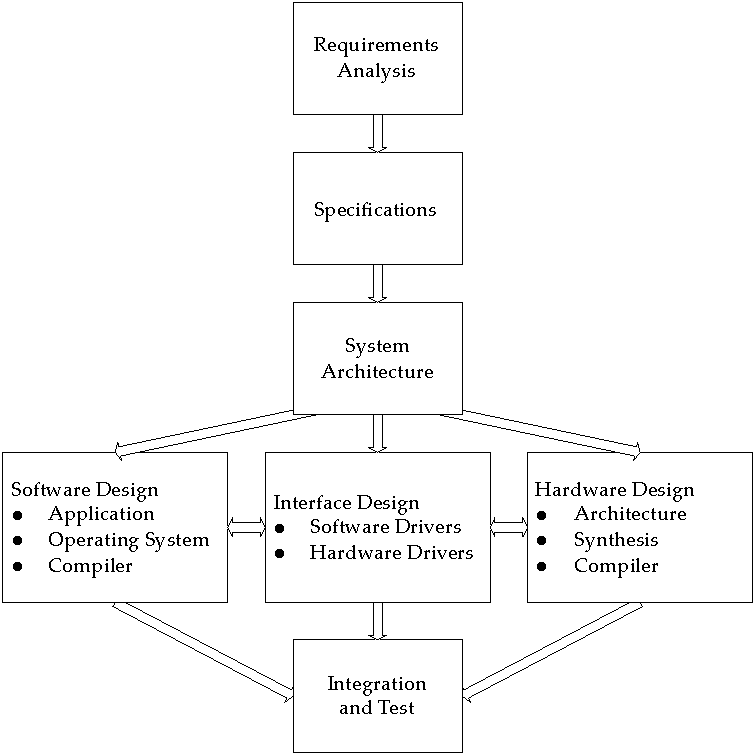
\includegraphics[width=3.8in,height=3.8in]{image5}
\caption{An embedded system design process {[}Ern97{]}.}
\label{figure:embedded DesignProcess}
\end{figure}

The field of software engineering is one in which the development of
different design process models is still under considerable flux today.
This is due to the complex nature of software and the failure of
computer scientists and engineers to effectively develop high-quality
software systems. There are many reasons why this is so. The sheer size
of software programs may easily exceed one million lines of code written
by many different software developers. One small mistake in those
millions of lines of code can cause the system to fail. Another
difficulty is in designing for upgrade and reuse of software. What if
the needs change after the millions of lines of code are developed and
one of the fundamental structures or objects needs to be upgraded?

The \emph{waterfall model} shown in Figure~\ref{figure:waterfallDesignProcess} 
is one of the first
proposed and most well-known software design processes. This is a
prescriptive model since the development proceeds linearly from the
first step where the user's needs are analyzed through the phases of
specification development, design, test, and maintenance. This works for
well-defined and moderately complex software applications, but fails as
complexity grows due to the inability to move between phases. A more
flexible and descriptive software design process is known as the
\emph{spiral model}, which is a cyclical process where phases are
revisited as necessary {[}Som01{]}. \emph{Extreme Programming} is a more
recent and controversial software development process, where relatively
small teams of software developers rapidly develop software following
some strict rules. Both the spiral model and Extreme Programming are
examined in more detail in the end of chapter problems.

\begin{figure}[h]
 
\includegraphics[width=4.6in,height=3.1in]{image6}
\caption{Waterfall software development process. In this
model, development proceeds linearly from requirements analysis, through
each subsequent phase, terminating with maintenance.}
\label{figure:waterfallDesignProcess}
\end{figure}

\section{The World-Class Engineer}\label{the-world-class-engineer}

The ability to effectively design is important for engineers, requiring
strong technical skills and an understanding of the design process. Yet,
this ability in itself is not enough to become an effective practicing
engineer. The Pennsylvania State University Leonhard Center for the
Advancement of Engineering Education, in consultation with a number of
industries, developed a description of what is referred to as a
``World-Class Engineer'' {[}Leo95{]}. Shown in Table~\ref{table:worldClassEngineer},
 the description identifies the characteristics of successful engineers, and
contains six major elements: 1) Aware of the World, 2) Solidly Grounded,
3) Technically Broad, 4) Effective in Group Operations, 5) Versatile,
and 6) Customer-Oriented. The description recognizes that engineers must
be effective in group operations, since the majority of projects are
carried out in teams. Not only that, many projects span multiple
technical disciplines and are executed in multifunctional organizations
that have diverse groups such as marketing, finance, human resources,
technical support, and service. It also recognizes that an engineer must
be versatile, innovative, understand ethical principles, and be
customer-oriented, important themes that are stressed throughout this
book.

\footnotesize
\begin{longtable}[c]{|m{14cm}|}
\caption{The World-Class Engineer (Copyright the Leonhard
Center for the Advancement of Engineering Education, The Pennsylvania
State University. Reprinted by permission.) 
\label{table:worldClassEngineer}}\\


\hline
\rowcolor{Gray}
\textbf{World Class Engineer} \\ \hline
\endfirsthead

\hline
\rowcolor{Gray}
{{\bfseries \tablename\ \thetable{} -- continued from previous page}} \\ \hline
\rowcolor{Gray}
\textbf{World Class Engineer} \\ \hline
\endhead
\endfoot

\hline

\begin{enumerate}
\itemsep0em 
\def\labelenumi{\Roman{enumi})}

\item Aware of the World 
\begin{itemize}
\itemsep0em 
\item  sensitive to cultural differences, environmental concerns, and ethical  principles
\item  alert to market opportunities (both high- and low-tech)
\item  cognizant of competitive talents, work ethic, and motivation
\end{itemize}

\item Solidly Grounded
\begin{itemize}
\itemsep0em 
\item  thoroughly trained in the fundamentals of a selected engineering
  discipline
\item  has a historical perspective and remains aware of advances in science
  that can impact engineering
\item  realizes that knowledge doubles at breakneck speed and is prepared to
  continue learning throughout a career
\end{itemize}

\item Technically Broad
\begin{itemize}
\itemsep0em 
\item  understands that real-life problems are multidisciplinary
\item  thinks broadly, seeing an issue in a rich context of various
  alternatives, probabilities, etc., rather than a narrow quest to find
  a single answer
\item  is conversant in several disciplines
\item  is trained in systems modeling and the identification of critical
  elements. Understands the need to design experiments to verify or
  extend analysis, as well as meet specification requirements
\item  is psychologically prepared to embrace any field necessary to solve
  the problem at hand
\end{itemize}

\item Effective in Group Operations
\begin{itemize}
\itemsep0em 
\item  cooperative in an organization of individuals working toward a common
  creative goal that is often multidisciplinary and multifunctional in
  nature
\item  effective in written and oral communication
\item   willing to seek and use expert advice
\item  cognizant of the value of time and the need to make efficient use of
  the time in all phases of an endeavor
\item   understanding and respectful of the many facets of business operation
  -\/- general management, marketing, finance, law, human resources,
  manufacturing, service, and especially quality
\end{itemize}

\item Versatile
\begin{itemize}
\itemsep0em 
\item  innovative in the development of products and services
\item  sees engineering as applicable to problem solving in general
\item  considers applying engineering beyond the typical employment focus of
  engineering graduates in the manufacturing industries, to the much
  broader economy (financial services, health care, transportation,
  etc.) where engineering skills could make a dramatic improvement in
  the productivity of those segments of the economy that employ 80
  percent of the U.S. population
\end{itemize}

\item Customer Oriented 
\begin{itemize}
\itemsep0em 
\item  realizes that finding and satisfying customers is the only guarantee
  of business success
\item  understands that products and services must excel in the test of
  cost-effectiveness in the global marketplace
\end{itemize}
\end{enumerate}
\\ \hline
\end{longtable}
\normalsize




\section{Book Overview}\label{book-overview}

Consider the digital camera, the cellular phone, and the space shuttle,
all complex systems that integrate a variety of technologies. A digital
camera is the synthesis of an embedded electronics system, optics, a
mechanical lens assembly, and the camera package itself. The embedded
electronics contain an imaging sensor, a digital display, digital
interface circuitry, flash memory storage, system control software, and
the user interface. The challenges of integrating the components of such
a system and having it record and transfer huge amounts of image data,
within an acceptable timeframe, are immense. Cellular phones are another
good example of a complex system that represents a technology that has
shrunk in size, but increased tremendously in functionality at the same
time. They encompass digital data communications, antenna design,
encryption for secure data transmission, a user interface display, and
Internet connectivity. At the other end of the spectrum are large-scale
space and military systems, such as the space shuttle. Despite the two
shuttle accidents, the safety and reliability requirements of the space
shuttle are incredibly high. Realizing such a system is accomplished by
a tremendous number of people from many disciplines working for
different organizations. All three of these technologies were developed
by large teams that encompass multiple disciplines. The processes and
practices employed in their development represent application of the
fundamentals that this book hopes to cover. While you won't be building
complete space shuttles by the end of this design course, you can expect
to apply design principles that allow you to design and integrate a
relatively complex system, maybe even a part of the space shuttle.


The intention is to teach the application of design principles to
computer and electrical engineers and to help prepare students for a
professional career. The majority of engineering education is devoted to
math, science, engineering science, and problem-solving. They are
important topics required to enter this highly technical field. However,
it is clear that there are other aspects beyond this that are equally
important for success, including an understanding of system design,
innovation, ethical principles, teamwork, and strong communication
skills.

The book is divided into three parts: I--Design Process, II--Design
Tools, and III--Professional Skills. This is shown in Figure~\ref{table:bookPhilosophy}
 as three separate, but related components that play a key role in achieving
Project Excellence---the ability to complete a project, in an ethical
manner that meets the customer's need, satisfies the constraints, and is
clearly communicated to all involved. The chapters are decoupled as much
as possible so that the reader can move between chapters as necessary.
In Part I, the emphasis is on understanding and gaining experience in
the different phases of the design process. The reader is guided through
the steps of project identification, research, specification
development, creative concept generation, and critical evaluation of
competing solutions. Part II addresses topics that are often employed in
design, including functional decomposition, description of system
behavior, reliability, and testing. Part III addresses professional
skills, including teamwork principles, project planning, ethics in
design and the profession, and oral communication skills.

\begin{figure}[h]
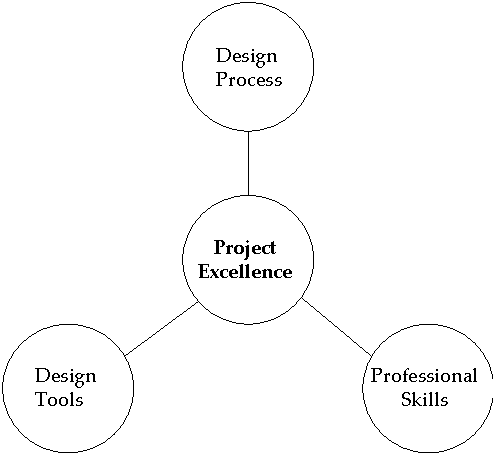
\includegraphics[width=2.875in,height=2.625in]{image7}
\caption{The guiding philosophy of this book. In order to
achieve success in executing engineering and design projects, it takes
an understanding of the design process, strong technical design tools,
and professional skills.}
\label{table:bookPhilosophy}
\end{figure}


Here are a few thoughts to conclude the chapter and get started on the
path to great designs. You are embarking on what will likely be a fun,
challenging, sometimes frustrating, and ultimately rewarding journey.
The systems that engineers work with continue to become increasingly
complex and multi-disciplinary in nature. The example problems presented
in this book come from the fields of analog electronics, digital
electronics, electrical systems theory, and software systems. These four
areas comprise a significant problem-domain common to the education of
most electrical and computer engineers. Finally, consider the quote
below by Robert Hayes on the importance of design.

Fifteen years ago, companies competed on price. Today it's quality.
Tomorrow it's design.---Robert H. Hayes, Harvard Business School, 1991.

What is this saying? Well, it is clear that the world continues to move
to a more knowledge-based society, where individuals and companies
compete on the strength of their intellectual capital and ability to
produce new and innovative products. That is what design is all about.
It is not saying that price and quality are unimportant, they certainly
are; in fact quality and reliability in design are part of this book. It
is that quality and price are a given, and successful products will be
distinguished by their design characteristics. The implication is that
design will play a larger role in the development and success of
products. The future Hayes predicted is now. Design is what
distinguishes between products that are seen as commodities and those
that are truly unique and profitable.

\section{Summary and Further
Reading}\label{summary-and-further-reading}

Engineering design is an iterative process in which the design team
employs creativity and technical knowledge to develop a solution that
best meets the end-users' needs within the constraints applied to the
problem. There is no single design process that can be applied to all
situations and technologies, but there are many common elements shared,
regardless of the technology under consideration. In order to
successfully bring designs to fruition, it takes a combination of design
tools, professional skills, and a clear understanding of the process
needed to complete designs. The objective of this book is to develop
your proficiency in these areas so that you may become an effective
engineer and achieve excellence in design projects.

\underline{Engineering Design Methods} by Nigel Cross {[}Cro00{]} presents the
differences between descriptive and prescriptive design processes, and
covers a wide array of processes in more detail. It also discusses the
cognitive characteristics of effective designers. There are many good
books on software engineering process development methods. \underline{Software
Engineering} by Ian Sommerville {[}Som01{]} discusses the different
software design process models, such as the waterfall and spiral models.
This is also true of many modern software engineering texts. The
original reference to the waterfall model is by Royce {[}Roy70{]}.
\underline{The Art of Innovation} by Michael Kelley {[}Kel01{]} describes the
activities of well-known design company IDEO and is a highly readable
description of their design practices. The ABC \emph{Nightline} news
program also produced an interesting segment on IDEO {[}ABC01{]} that
can be purchased at the ABC website. \underline{The Circle of Innovation} by
Tom Peters {[}Pet97{]} is another popular book that provides his
perspective on current trends in business and the importance of design.

\section{Problems}
\label{problems}

\begin{enumerate}
\itemsep0em 
\def\labelenumi{\arabic{enumi}.}
\item
  In your own words, describe the difference between prescriptive and
  descriptive design processes. Cite examples of each.
\item
  Describe the relationship between the Problem Identification,
  Research, and Requirements Specification phases of the design process.
\item
  Describe the relationship between the Concept Generation and Design
  phases of the design process.
\item
  Construct a prescriptive design process for the Problem
  Identification, Research, Specification, Concept, and Design phases of
  the design process. The result should be a flow chart that contains
  decision blocks and iteration as necessary.
\item
  Describe the main differences between the VLSI and embedded system
  design processes.
\item
  Using the library or Internet, conduct research on the spiral software
  design process.

\begin{enumerate}
\itemsep0em 
\def\labelenumi{\alph{enumi})}
\item
  Outline the significant elements of the spiral software design
  process.
\item
  Describe the advantages and disadvantages of this relative to the
  waterfall model?
\end{enumerate}

\begin{quote}
Cite all reference used.
\end{quote}

\item
  Using the library or Internet, conduct research on the Extreme
  Programming design process.

\begin{enumerate}
\itemsep0em 
\def\labelenumi{\alph{enumi})}
\item
  Outline the significant elements of the Extreme Programming paradigm.
\item
  What are the pro and con arguments for this software development
  model?
\end{enumerate}

\begin{quote}
Be sure to cite references.
\end{quote}

\item
  \textbf{Project Application.} In preparation for project and team
  selection, develop a personal inventory that includes a list of five
  favorite technologies or engineering subjects that you are interested
  in pursuing. Also, list the strengths and weaknesses that you bring to
  a project team.
\end{enumerate}


\chapter{Project Selection and Needs Identification}
\graphicspath{ {./chapter02/Fig} }

\begin{itquote}
For every problem there is a solution that is simple, neat, and
wrong.---H.L. Mencken
\end{itquote}

Traditionally, companies have organized resources based on functions
such as accounting, engineering, finance, manufacturing, and marketing.
It is often more effective to organize around projects that are of
significant value and align resources to meet the needs of the project.
This means that traditional departments and middle management are being
de-emphasized and the role of projects is growing. Capstone design
projects provide a great opportunity to gain experience in the
management and execution of a project. One of the first and most
important decisions encountered is selecting a project to pursue.

The objective of this chapter is to provide pragmatic guidance in the
project selection phase. A description of design and engineering
projects is presented, followed by advice on how projects can be
selected by engineering students who wish to put design principles into
practice. The chapter addresses how to identify the needs of the
end-user and provides guidance for conducting background research. All
of this information is brought together in a Problem Statement that
identifies the needs, the goals of the project, and research on the
technology.

\section*{Learning Objectives}
\noindent\rule{\linewidth}{1pt}
By the end of this chapter, the reader should:
\begin{itemize}
\item
  Have an understanding of the types of projects that electrical and
  computer engineers undertake.
\item
  Understand and be able to apply criteria for project selection.
\item
  Know how to determine, document, and rank end-user needs.
\item
  Be aware of resources available for conducting research surveys.
\item
  Have selected a project concept and developed a Problem Statement.
\end{itemize}

\section{Engineering Design Projects}
\label{section:engineering-design-projects}

This section provides a classification of design and describes some of
the types of projects undertaken by practicing engineers and those
tackled in student projects. In reality, most projects don't fit neatly
into the categories presented, but are some combination of them. The
objective of a design project is to create a new
\emph{\textbf{artifact}} (system, component, or process) to meet a given
need. Within the design domain there are different types of designs that
are classified broadly into three categories of Creative, Routine, and
Variant designs {[}Cro00{]}.

\emph{\textbf{Creative designs}} represent new and innovative products.
An example of a creative design is the Palm Pilot Personal Digital
Assistant (PDA). While the idea for the PDA had been around for awhile,
earlier attempts at developing the technology, notably the Apple Newton,
were unsuccessful. This was primarily due to unreliable handwriting
recognition that frustrated the user. However, Palm Computing had the
creative idea to develop a simplified handwriting language, Graffiti,
which eliminated the need for natural handwriting recognition. The Palm
Pilot is a great example of a creative design---it is simple (four basic
functions), fits in your pocket, and is easy to use. This innovation
spawned a huge hand-held computing industry.

\emph{\textbf{Variant designs}} are variations of existing designs,
where the intent is to improve performance or add features to an
existing system. Many engineering projects fall into this category. For
example, the objective may be to increase accuracy or system throughput.

\emph{\textbf{Routine designs}} represent the design of devices for
which theory and practice are well-developed. Examples are DC power
supplies, analog and digital filters, and basic digital components such
as adders and comparators. Routine designs are often components of more
complex creative and variant designs.

Within these three categories of design, there are many different types
of projects. \emph{Systems engineering and systems integration projects}
represent the synthesis of many subsystems into a larger system. They
may be creative or variant designs, but have unique challenges since
they are typically large and involve many people and technologies.
Adherence to good design processes is important for their success.
Engineers are often engaged in \emph{systems test}, where the objective
is to ensure that a system meets stated requirements and the needs of
the user. Examples include the testing of systems for use in space and
military environments.

The objective in \emph{experimental design} \emph{projects} is to design
experimental procedures and apparatus for determining the
characteristics of a system. For example, an engineering team may test a
system under a variety of operating conditions. Example 2.3 presented
later in the chapter is such a project, where the objective was to
design a series of experiments to test the feasibility of gigabit
Ethernet technology in a military environment. The test explored the
impact of environmental factors such as temperature and vibration, and
further used this data to estimate the operating lifetime of the
Ethernet board. Upon completion of this project, the team made
recommendations as to the allowable operating ranges of the technology.

The objective in \emph{analysis projects} is to analyze some aspect of
an existing system to improve or correct it. For example, a system or
process may be failing in the field and the source of the failure
unknown. Tools such as the Failure Mode Effects and Analysis technique
may be applied in this situation to identify the sources of failure. In
t\emph{echnology evaluation} \emph{projects}, technologies are assessed
to determine if they can be used in a given application. This may be to
determine if the technology can improve an existing system, or to
characterize its operating performance.

The objective of a \emph{research project} is to perform research or
experiments with the goal of discovering or creating a new technology.
The fundamental difference between this and other types of projects is
that the ultimate outcomes are unknown. Most engineering research falls
under the category of \emph{applied research}. This refers to the
creation of new technology or systems based on existing technology and
theory developed from fundamental research. \emph{Fundamental research}
emphasizes the discovery of new scientific principles without
necessarily having an intended application. Fundamental research is very
valuable, but not typically a part of design projects.

\section{Sources of Project Ideas}
\label{section:sources-of-project-ideas}

Depending upon your situation, you may have the opportunity to identify
and select your project. The list below provides some places to search
for project ideas:

\begin{itemize}
\item
  \emph{Industry sponsored projects.} Many companies will sponsor
  projects and are happy to do so, particularly if you have worked for
  them on an internship.
\item
  \emph{Engineers without Borders
  (\href{http://www.ewb-usa.org}{www.ewb-usa.org})}. This organization
  sponsors student projects to improve the quality of life in developing
  countries.
\item
  \href{http://www.FreeRandD.com}{\emph{www.FreeRandD.com}}. This is a
  clearinghouse for businesses and students teams to collaborate on
  projects. It allows businesses to post capstone project ideas for
  students to work on, while students can post resumes and project
  interests.
\item
  \emph{Your campus and local community.} In our school, a number of
  student teams have identified novel projects by asking other
  departments on campus for ideas. They have also been successful in
  approaching local community organizations for ideas, such as museums
  and research institutes.
\item
  \emph{Brainstorm.} Get together with a group of your peers and
  brainstorm on project ideas. You will be surprised at how many project
  ideas you can develop in a good brainstorming session (see Chapter 4).
  Do not only consider project ideas, but also brainstorm to identify
  problems that need solutions.
\end{itemize}

\section{Project Feasibility and Selection Criteria}
\label{section:project-feasibility-and-selection-criteria}

This section provides questions to consider when examining the
feasibility of a project. George H. Heilmeier (an electrical engineer
who has held positions as Chief Technology Officer of Texas Instruments,
Director of the Defense Advanced Research Projects Agency, and CEO of
Bellcore) developed a set of questions to answer when starting a new
project {[}Sha94{]}. Heilmeier argued that all projects must be tied to
the goals of the organization, and applied this by asking the following
questions:

\begin{itemize}
\item
  What are you trying to do? Articulate your goals using absolutely no
  jargon.
\item
  How is it done today, and what are the limitations of current
  practice?
\item
  What is new in your approach, and why do you think it will be
  successful?
\item
  Who cares? If you are successful, what difference will it make?
\item
  What are the risks and payoffs?
\item
  How much will it cost? How long will it take?
\item
  What are the midterm and final exams to check for success?
\end{itemize}

Heilmeier credits successful completion of projects that he managed to
answering these questions up-front and adhering to disciplined project
management processes.

A second perspective is offered from an organizational project
management viewpoint {[}Gra02{]} that provides the following criteria
for project selection:

\begin{itemize}
\item
  \emph{The project must be tied to the mission and vision of the
  organization.} Believe it or not, organizations often spend resources
  fruitlessly on projects that don't meet this criterion. To be fair,
  there is always risk associated with a project and it is sometimes
  hard to judge exactly how well a project meets this criterion. For
  engineers who are new to an organization, it is hard to judge a
  project's importance relative to the mission and goals, but if you
  find yourself in this situation, do not be afraid to ask some
  questions. Novices ask basic questions that are often overlooked by
  those who are highly experienced or intimately involved in a project.
\item
  \emph{Must have payback.} An economic analysis should be done to
  estimate if the project will make a profit. Much of this is outside
  the scope of this text, requiring marketing and financial analyses.
  Chapter 10 covers the basics of project cost estimation that will help
  in trying to answer this question.
\item
  \emph{Should have selection criteria.} Sound criteria for selecting
  among competing projects should be employed. The example at the end of
  this section demonstrates the application of criteria in project
  selection.
\end{itemize}

\begin{itemize}
\item
  \emph{Objectives of the Project should be SMART: Specific, Measurable,
  Assignable, Realistic, Time-Related}. Chapter 3 addresses how to
  determine project requirements that are Specific and Measurable.
  Assignable, Realistic, and Time-Related all refer to project
  management aspects that are covered in Chapter 10. The objective is to
  develop tasks that are assigned to groups or individuals and
  realistically can be completed in the given timeframe.
\end{itemize}

The following example demonstrates how to apply a project selection
model using a method known as the Analytical Hierarchy Process. AHP is a
decision making method that is described in Appendix B and is utilized
frequently throughout the text -- \textbf{the reader should read
Appendix B prior to proceeding with this example}.

\cbstart

\textbf{Example 2.1} A project selection model for capstone design.

Assume that you are part of a capstone design team that has the
opportunity to select their project from competing project ideas. The
steps in making a decision using AHP are to select the criteria that
drive the decision, determine relative weights of the criteria, rate the
alternatives (in this case project concepts) against the criteria, to
compute a weighted score for each of the alternatives, and then review
the decision.

\ul{Step 1: Determine the selection criteria}

To select the criteria, assume that the team brainstorms to determine
the following criteria that interest the team members:

\begin{quote}
A -- Match to team skills

B -- Technical complexity

C -- Creativity

D -- Market potential

E -- Industry sponsorship
\end{quote}

\ul{Step 2: Determine the criteria weightings}

Assume the team applies the method of pairwise comparison to determine
the weights as shown in Appendix B. In order to do so, the team
systematically compares each criterion to all others using the following
scale of relative importance:

1 = equal, 3 = moderate, 5 = strong, 7 = very strong, 9 = extreme.

Again, details of pairwise comparison are outlined in Appendix B and the
results are below. \\


\begin{tabular}{ |> {\columncolor{Gray}} c  |c|c|c|c|c|c|} 
\hline
\rowcolor{Gray}
Criteria & A & B & C & D & E & Weight \\ 
\hline
A & 1 & 5 & 5 & 3 & 3 & 0.52 \\
\hline
B & 1/5 & 1 & 3 & 1/3 & 1/3 & 0.12 \\
\hline
C & 1/5 & 1/3 & 1 & 1 & 3 & 0.09 \\
\hline
D & 1/3 & 3 & 1 & 1 & 5 & 0.18 \\
\hline
E & 1/3 & 3 & 1/3 & 1/5 & 1 & 0.09 \\
\hline
\end{tabular}
\\

This is an important step and one often overlooked -- the team has
identified what is important to it in project selection. It is clear
that match to the team skills (criterion A) is most important, by a
large margin, followed by market potential.

\ul{Step 3: Identify and rate alternatives relative to the criteria}

Assume that the team identifies three potential projects ideas: 1 --
IEEE sponsored robot competition, 2 -- Industry sponsored project to
design a new test protocol, and 3 -- Design of an item-finder device to
help people locate lost items. Furthermore, the team goes through the
process of rating each project relative to the criteria as outlined in
Appendix B. These ratings are reflected in the decision matrix in the
next step.

\ul{Step 4: Compute scores for the alternatives}

The decision matrix below is constructed and the scores for the
alternatives determined.


\begin{tabular}{|l|c|c|c|c|}
\hline
\rowcolor{Gray}
\multirow{ 2}{*}{Selection Criteria} & \multirow{ 2}{*}{Weights} & \multicolumn{3} {|c|} {Alternatives} \\ \hline

\rowcolor{Gray}
                                                           &                                              & Project 1 & Project 2 & Project 3 \\ \hline
A (Match to skills) & 0.52 & 0.40 & 0.20 & 0.40 \\  \hline
B (Technical Complexity) & 0.12 & 0.40 & 0.30 & 0.30 \\ \hline
C (Creativity) & 0.09 & 0.45 & 0.20 & 0.35 \\ \hline
D (Market potential) & 0.18 & 0.05 & 0.35 & 0.60 \\ \hline
E (Industry sponsorship) & 0.09 & 0.00 & 1.0 & 0.00 \\ \hline
Score & & 0.31 & 0.31 & 0.38 \\ \hline
\end{tabular}


\ul{Step 5: Review the decision}

Project 3 (item finder) is rated the highest among the three choices
based upon the weights determined by the team members. It is a good
match to the team skills, but also matches their desire to solve a
problem with good market potential. The remaining two projects are rated
about equal.
\cbend

\section{Needs Identification}
\label{section:needs-identification}

Often a customer, client, or supervisor comes to you with a problem to
solve and you must determine the needs or requirements for the solution
to the problem. In other words, determine the \emph{voice of the
customer}. This seems like a simple statement---ask the customer what
they want and you are done, right?

As an illustration, let's say a client comes to you with the following
request---\emph{The traffic at the front of campus is too congested. I
would like you to design a new traffic lane for northbound traffic
exiting at the intersection at the front of the college.} So you design
this new lane and have it added to the intersection. However, you find
out three months later that the traffic congestion has decreased a
little bit, but it is still a significant problem. So what went wrong?
Clearly you did what was asked of you, but the problem was not solved,
meaning that you were solving the wrong problem. The real problem was to
improve the flow of traffic at the entrance. In this case, the client
gave both the problem and the solution all in one statement. That is
fine if a careful feasibility study was done and it was known that the
additional traffic lane would alleviate the problem, but that was not
the case here. This hypothetical situation is not so far fetched and
happens in practice via neglect to do the up-front research or because
underlying assumptions change. The point is that the \ul{correct}
problem should be identified and solved.

It would be better if the client had simply asked to improve the traffic
flow, providing the opportunity to analyze the situation and develop
different design options. Some questions to be asked in this situation
are: \emph{How much additional traffic is there? At what times does this
happen? Where is the traffic coming from? What is an acceptable waiting
time at the intersection?} It may be that several new lanes are needed,
or perhaps the sequencing of the traffic signals is wrong, or maybe a
new entrance could be added for less cost and improved traffic flow.

The lesson is that customers often come with the problems and solution
all wrapped up together. When this is done, the \emph{\textbf{design
space}}, the space of all possible solutions to the problem, is
unnecessarily limited. Be ready to tactfully challenge the assumptions
and ask questions to get to the root of the problem. Ask clarifying
questions, analyze, pick apart the request, and focus on the problem,
not the solution.

Researchers and practitioners have examined the problem of eliciting
needs, and it is an important pre-requisite for developing good
engineering requirements specifications. Ulrich and Eppinger {[}Ulr03{]}
proposed a process for obtaining the \emph{voice of the customer} using
the following five steps: 1) Gather raw data from users; 2) Interpret
raw data in terms of needs; 3) Organize needs into a hierarchy; 4)
Determine the relative importance of the needs; and 5) Review the
outcomes and the process. Each of these steps is described in the
following sections.

\subsection*{ Step 1: Gather Raw Data from Users}

\textbf{DILBERT\textsuperscript{®} by Scott Adams}

\begin{figure}[h]
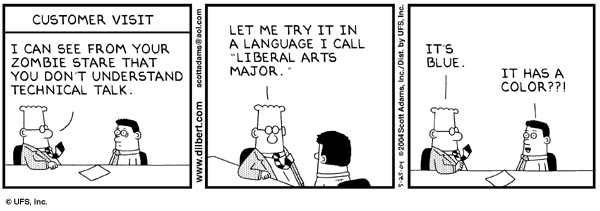
\includegraphics[width=5.5in,height=1.9in]{image1.png}
\caption{ The difficulties of communicating with the customer. (Dilbert © United Feature Syndicate. Reprinted by
permission.)}
\label{figure:dilbertCommunication}
\end{figure}


This is often accomplished via interviews with supervisors, key users,
or people from the client organization. In cases where new products are
being developed, focus groups are often employed. The advantage of
interviews and focus groups is that they provide the opportunity for
dialogue with the user where new ideas, concepts, and needs may emerge.
Another option is direct observation, where the team goes out and
examines the system in use and develops concepts for improving it. IDEO
Corporation is an innovative and successful company that designs new
products and systems. They rely heavily on direct observation as a
technique for successfully developing innovative products {[}Kel01{]}.
For example, IDEO was asked by a client to develop a new medical
instrument for balloon angioplasty used in hospital operating rooms. A
critical requirement from the user was that only one hand could be used
to operate the device because the technician's other hand had to be free
during the procedure. From direct observation, the IDEO design team
found that even though the current system was designed for one-hand use,
it was impractical, and the technicians actually used both hands. IDEO
designed and developed a two-handed pump that not only worked better
than the one handed pump, but was quieter, easier to read, and had
increased precision. This is another example of the customer specifying
the solution as part of the problem statement.

Ulrich and Eppinger provide the following questions to ask during an
interview:

\begin{itemize}
\item
  When and why do you use this type of product (system)?
\item
  Walk us through a typical session using the product.
\item
  What do you like about the existing products?
\item
  What do you dislike about the existing products?
\item
  What issues do you consider when purchasing the product?
\item
  What improvements would you make to the product?
\end{itemize}

\subsection*{Step 2: Interpret the Raw Data in Terms of Needs}


In this step the raw data is translated into customer needs. The needs
are expressed in terms of what the system must do (a requirement) as
opposed to how it is done. Statements of the customer's needs are known
as \textbf{\emph{marketing requirements}} or \emph{\textbf{marketing
specifications}}. For example, ``\emph{The system should have
high-quality audio}'' is a need or marketing requirement from the
customer regarding performance, but says nothing about how it will be
achieved. Marketing requirements are short sentences that describe the
need in the language of the customer. They typically do not have a
numerical target and are described as a state of being for the system.
Other examples of marketing requirements are, ``\emph{The system should
be easy-to-use,}'' and ``\emph{The system should be able survive a drop
from the runner's height.}''

\subsection*{Step 3: Organize Needs into a Hierarchy}

The marketing requirements are organized into a hierarchy of needs
arranged from the most general to the most specific in successive levels
of detail as required by the problem. It is organized by functional
similarity, not as hierarchy of importance (that is the next step). This
hierarchy is referred to as an \emph{\textbf{objective tree}}. An
example objective tree for a portable audio device intended for use by
runners is shown in Figure~\ref{figure:audioPortable}. The three high-level objectives
determined were high-quality audio, portable, and easy-to-use. Each of
these is further sub-divided into the characteristics that support the
higher level. For example, portability is divided into the needs of
lightweight, small, ergonomic, and the ability to operate in the
environment. The environmental need is further expanded into needs that
support it.

\begin{figure}[h]
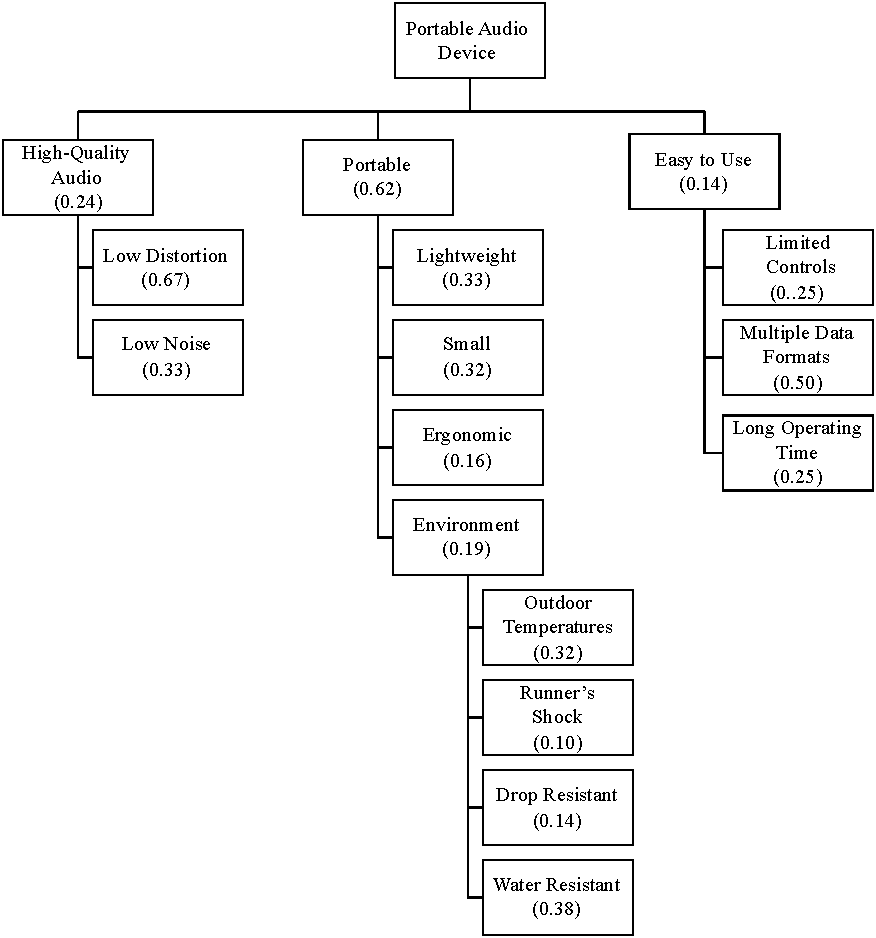
\includegraphics[width=5.2in,height=5.6in]{image2}
\caption{Objective tree for a portable audio device to be
used by runners. The weights reflect the relative importance of needs at
each level in the hierarchy as determined in Step 4 of the
process.}
\label{figure:audioPortable}
\end{figure}

\subsection*{Step 4: Determine the Relative Importance of the Needs}


The relative importance of the needs is determined based upon the user
needs. As we saw in Example 2.1 and as presented in Appendix B, the
pairwise comparison is a good technique for determining relative
importance and weighting of needs. In pairwise comparison, all needs are
systematically compared to all other needs at the same level in the
hierarchy. An example pairwise comparison table for this problem is
shown in Table~\ref{table:highQualityAudio} 
with the resulting weights for each need indicated.
This shows that portability is the most important need, followed by
audio quality and ease-of-use. The weights are also reflected in the
objective tree in Figure~\ref{figure:audioPortable}. In addition, the needs at each sublevel in
the hierarchy are compared, the results of which are reflected in 
Figure~\ref{figure:audioPortable}. The rankings are used in later chapters to compare design
alternatives.

\begin{table}[h]
\centering
\begin{tabular} {|> {\columncolor{Gray}} l|c|c|c||c|}
\hline
\rowcolor{Gray}
                             & High-Quality Audio & Portable & Easy-to-Use & Weight \\
\hline
High-Quality Audio & 1 & 1/3 & 2 & 0.24 \\
\hline
Portable & 3 & 1 & 4 & 0.62 \\
\hline
Easy-to-Use & 1/2 & 1/4 & 1 & 0.14 \\
\hline
\end{tabular}
\caption{Pairwise comparison matrix for ranking the
highest-level needs of the portable audio device. This comparison should
be carried out for all levels of the objective tree.}
\label{table:highQualityAudio}
\end{table}


\subsection*{Step 5: Review the Outcomes and the Process}

The design process and all of its sub-processes are methods for making
good decisions, and this technique for needs identification is no
different. There is a certain amount of subjectivity and judgment that
goes into it; the end result should be reviewed to determine if it makes
sense. The objective is to challenge assumptions, fully identify the
problem, and make informed decisions.

The three outcomes of this process are the marketing requirements that
identify the needs, an objective tree that provides a hierarchical
representation of the needs, and a ranking of the relative importance of
needs. This process may seem as though it does not apply to student
design projects, but in reality it does. The questions in this chapter
are certainly candidates to ask when working on company-sponsored
projects. If it is not a company sponsored project, the user needs
should still be considered. For example, questions can be asked of
friends and co-workers who are potential users of the system, focus
groups can be formed, surveys administered, and Internet bulletin boards
and discussion groups employed to gather this information.

\section{The Research Survey}
\label{section:the-research-survey}

It is important to conduct a thorough research survey while defining the
project concept. Failure to do so may translate into time and money
spent reinventing the wheel, while not taking full advantage of existing
components, knowledge, practices, and technology. During the research
phase, competing systems and technologies are identified, and based upon
them the project concept refined, or in some cases abandoned. The
character and strategy of the research survey is driven by the nature of
the project. In general, the objective is to develop an understanding of
the underlying scientific principles and demonstrate a familiarity with
the state-of-the-art in the particular field. Some questions to be
answered in the research survey are:

\begin{itemize}
\item
  What is the basic theory behind the concept?
\item
  How is it currently being done?
\item
  What are the limitations of current designs or technology?
\item
  What are the similarities and differences between your concept and
  existing technologies?
\item
  Are there existing or patented technologies that may be relevant to
  the design? If so, what are they and why are they relevant?
\end{itemize}

\textbf{Internet Searching}

The Internet is a powerful, fast, and readily accessible source for
conducting research. There are many excellent search engines for
locating web resources, but understand that it is important to go beyond
the well-known search engines and beyond the Internet in the survey.

One of the risks, and also one of the wonderful things, about the
Internet is that virtually anybody can post information. It is important
to analyze websites to ensure that they are reliable and credible. There
are resources available that provide pointers on how to evaluate this
credibility {[}Mci02, Sch98{]}, and a little common sense goes a long
way. One of the important things to look for is authorship---the author
should be clearly identified and any affiliations listed. Carefully
determine whether the information is subjective opinion or possibly a
commercial for a product. Credible sites should provide references to
original sources of material. Another step is to verify website content
in print media or other reliable sources.

There are thousands of search engines available, making the task of
selecting one challenging. Also, there are different types of search
engines: text (search for the text or keywords; subject heading or
full-page text search), indexed (information categorized into
directories), meta-search (engines that search other engines), and
natural language processing (allowing natural language queries). A
listing of search engines to try are
\href{http://www.altavista.com}{www.altavista.com},
\href{http://www.AskJeeves.com}{www.AskJeeves.com},
\href{http://www.google.com}{www.google.com},
\href{http://www.kartoo.com}{www.kartoo.com}, and
\href{http://www.yahoo.com}{www.yahoo.com}. The Librarian's Index to the
Internet, \href{http://www.lii.org}{www.lii.org} is a collection
selected and evaluated by librarians, and according to their website, it
is \emph{a} ``\emph{well-organized point of access for reliable,
trustworthy, librarian-selected Internet resources}.'' This information
may change rapidly and represents current information at the time of
publication.

\textbf{Electrical and Computer Engineering Resources}

Realize that the major search engines will not find all information
available on the Internet. There are many websites with specialized
search capabilities related to electrical and computer engineering
design.

\begin{itemize}
\item
  EE Product Center,
  \href{http://www.EEProductCenter.com}{www.EEProductCenter.com}. A
  website for locating electronic components and their manufacturers. It
  provides links to product datasheets and application notes. It has a
  keyword search engine and a tree structure search for finding
  components. For example, you can start with Op Amps and delve into
  sub-categories such as Precision and High-Speed.
\item
  Circuit Cellar,
  \href{http://www.CircuitCellar.com}{www.CircuitCellar.com}. This
  companion website for the magazine is a great reference for designers.
  It emphasizes embedded systems and electronics projects with many
  tutorial articles and project ideas.
\item
  Datasheet Catalog,
  \href{http://www.DatasheetCatalog.com}{www.DatasheetCatalog.com}. A
  datasheet source for electronic components and semiconductors.
\item
  Dr. Dobbs, \href{http://www.ddj.com}{www.ddj.com}. The magazine and
  companion website are a resource for software developers that includes
  tips and tutorials.
\item
  EE Times, \href{http://www.EETimes.com}{www.EETimes.com}. Industry
  newspaper for electrical engineering field with information on current
  technology developments.
\item
  Electronic Design Magazine,
  \href{http://www.EDNmag.com}{www.EDNmag.com}. This is free magazine
  for electrical design engineers that provides information on the
  latest products. The website has a number of categorized technical
  resources and a design ideas section.
\item
  ON Semiconductor, \href{http://www.OnSemi.com}{www.OnSemi.com}. ON
  Semiconductor is a supplier of semiconductors for a wide range of
  applications, with a particular emphasis on power management. The
  website has a searchable database of over 15,000 components, and
  provides guidelines for component selection based on different
  applications.
\item
  The Thomas Register,
  \href{http://www.ThomasRegister.com}{www.ThomasRegister.com}. This is
  a source for finding companies and products in North America. It
  allows searches for parts and equipment that may be used in a design
  project. It provides profiles of companies that meet the search
  criteria and describes the products they make.

  In addition, most manufacturers of electronic components have websites
  providing product datasheets and application notes for their products.
  Application notes demonstrate how to use components in real
  applications. Examples are Dallas Semiconductor, Fairchild
  Semiconductor, Motorola, and Texas Instruments.
\end{itemize}

\textbf{Government Resources}

\begin{itemize}
\item
  US Bureau of Labor Statistics, \url{http://stats.bls.gov}. This has
  valuable information on consumer spending information, allowing one to
  determine things such as how much people spend and what they spend it
  on. It also profiles specific industries and forecasts employment in
  different industry sectors.
\item
  US Government Official WebPortal,
  \href{http://www.FirstGov.gov}{www.FirstGov.gov}. This is an entrance
  to all US government web resources.
\item
  US Patent Office, \href{http://www.uspto.gov}{www.uspto.gov}. A
  searchable database of all patents back to 1790. Full text searches
  are available back to 1976 and full images back to 1790. It has
  information on the basics of patents, trademarks, and copyrights.
\end{itemize}

\textbf{Journal and Conference Papers}

The search should include journal and conference papers if technically
detailed information on the latest theory or applications is needed.

\begin{itemize}
\item
  ACM (Association for Computing Machinery) Digital Library,
  \href{http://www.acm.org}{www.acm.org}. Provides abstracts (full text
  for subscribers) for ACM journals and conference proceedings.
\item
  Compendex,
  \href{http://www.engineeringvillage2.org}{www.engineeringvillage2.org}.
  This provides indices to journal and conference papers in a broad
  scope of engineering fields, referencing material back to 1970.
\item
  IEEE (Institute of Electrical and Electronics Engineers) Xplore
  Electronic Library, \href{http://www.ieee.org}{www.ieee.org}. Provides
  abstracts (full text for subscribers) to all IEEE journals,
  transactions, magazines, and conference subscriptions published since
  1988. Abstracts for all IEEE standards are publicly available.
\end{itemize}

\section{Needs and Objectives Statements}
\label{section:needs-and-objectives-statements}

Two parts of the Problem Statement are the needs and objectives
statements. The \emph{needs statement} identifies and motivates the need
for the project and should:

\begin{itemize}
\item
  Briefly and clearly state the need being addressed.
\item
  Not provide a solution to the problem.
\item
  Provide supporting information collected as outlined in Section 2.4.
\item
  Provide any supporting statistics and anecdotes that support the need.
\item
  Describe current limitations.
\item
  Describe supporting processes that are needed to understand the need.
  This is particularly important in industry-sponsored projects having
  specific needs that may not be clear to the average person.
\end{itemize}

The \emph{objectives statement} typically ranges from one or two
sentences to one or two paragraphs in and should:

\begin{itemize}
\item
  Summarize what is being proposed to meet the need.
\item
  Provide some preliminary design objectives (detailed requirements are
  developed later).
\item
  Provide a preliminary description of the technical solution, avoiding
  a detailed description of the implementation. Often the input and
  output behavior of the system are described. The complete solution is
  not usually posed until after the engineering requirements are fully
  determined.
\end{itemize}

Example needs and objectives statements are provided in Examples
2.2--2.4.

\cbstart
\textbf{Example 2.2} iPod Hands-Free Device Needs and Objectives.
\emph{Abstracted from the iPod Hands-Free Device Design Report by
Al-Busaidi, Bellavia, and Roseborough {[}Alb06{]}.}

\ul{Need:} According to AppleInsider, approximately 10.3 million people
owned iPods at the end of 2004 and many of the owners used them while
operating their automobiles. The National Highway Traffic Safety
Administration estimates that driver distraction is a contributing cause
of 20 to 30 percent of all motor vehicle crashes -- or 1.2 million
accidents per year. One research study has estimated that driver
inattention may cause as many as 10,000 deaths each year and
approximately \$40 billion in damages. iPods can present a distraction
to drivers that is similar to cell phones in that the driver's attention
is divided between controlling the steering wheel, watching the road,
and navigating controls on the iPod. A system is needed to allow users
to navigate among the music selections of their iPod without distracting
their attention from the road.

\ul{Objective:} The objective of this project is to design and prototype
a device that will make the iPod safer to use while driving an
automobile, by allowing hands-free control of the iPod. The device will
interact with the user using spoken English commands. The user will be
able to issue simple voice commands to the device to control the
operation of the iPod. In turn, the device will communicate information
verbally, such as song titles that are displayed on the iPod screen, to
the user.
\cbend

\hphantom  \\

\cbstart

\textbf{Example 2.3} Experimental Design Problem Needs and Objectives.
\emph{Abstracted from the Intel Pro 1000XF Server Testing Design Report
by Esek, Hunt, and Lewis. {[}Ese03{]}.}

\ul{Need:} Our industry sponsor is investigating the performance of
commercial grade gigabit Ethernet fiber optic equipment for computer
data communications in a military environment. The proposed system will
utilize an Intel Pro1000 XF server card. This is a harsh operating
environment and its effects on the performance and lifetime of the
equipment are unknown. The client wishes to understand how the military
environment affects the optical power margin of the Intel Pro 1000 XF
card and associated connectors and cabling.

\ul{Objective:} The goal of this project is to design the experimental
equipment and test procedures to determine the effects of temperature
variations and vibration on the optical power margin and the operating
lifespan of the system.
\cbend

\hphantom  \\

\cbstart

\textbf{Example 2.4} Portable Aerial Surveillance Needs and Objectives.
\emph{Abstracted from the PASS Design Report by Andre, Kolb, and Thaler
{[}And06{]}.}

\ul{Need:} Emergencies happen all across the world, all of the time.
There are nearly 2,000,000 reported fires in the United States every
year, and over 90 tactical activations of Pennsylvania's Special
Emergency Response Team which handles barricaded suspects and hostage
situations. There have been over 100 documented riots in the United
States in the past century, with the Los Angeles Riot alone causing \$1
billion in damage. Having an aerial view of these situations would be a
great benefit to the emergency workers on the ground. For example,
police may have to monitor a large crowd or a hostage situation where
aerial surveillance would allow them to observe the situation from a
safe distance and use the footage as evidence in court. Firefighters
could use aerial surveillance to examine fire damaged buildings and
search for victims through the windows of high-rise buildings. In large
cities, emergency organizations often employ helicopters for aerial
surveillance. However, in smaller rural towns, helicopters either take
too long to reach the scene from a nearby city or they are too expensive
to afford. The least expensive two-seat helicopters cost over \$400,000,
while new helicopters cost well over a million dollars with average
operating costs of \$400-\$1000 per hour. There is a need for a low cost
aerial device that can provide emergency workers with overhead
surveillance of emergency situations.

\ul{Objective:} The objective of this project is to design a device that
will provide emergency workers with a live aerial view of a situation at
a cost that small municipalities can afford. The device will deploy
rapidly and record and log video. The camera will also include pan and
zoom functionality to make identification of victims and suspects
easier.
\cbend

\section{Project Application: The Problem Statement}
\label{section:project-application-the-problem-statement}

A format for a Problem Statement that integrates the elements of this
chapter is as follows:

\begin{itemize}
\item
  \emph{Need.} A statement that identifies the needs of the project.
\item
  \emph{Objective.} Describes the concept proposed to meet the needs
  identified.
\item
  \emph{Background.} A summary of the research survey on the relevant
  technologies and systems. The objective is to provide an introduction
  answer the questions posed in Section~\ref{section:needs-identification}. 
  The length and content of
  this section varies depending upon the project.
\item
  \emph{Marketing Requirements.} Short statements describe the user
  needs.
\item
  \emph{Objective Tree}. A hierarchical representation of the needs
  based on functional similarity with the relative weights of the needs
  identified.
\end{itemize}

\section{Summary and Further Reading}
\label{section:summary-and-further-reading}

This chapter addressed the types of projects that are often undertaken
by engineers and provides guidance in terms of questions to ask when
selecting a project. The success of design projects depends upon
adequately determining the user's needs and desires for the system. A
process developed by Ulrich and Eppinger for needs elicitation was
presented. The three outcomes of this process are: 1) marketing
requirements identifying the customer needs, 2) an objective tree that
hierarchically represents the needs, and 3) a ranking of the relative
importance of the needs. It is important to conduct research on the
concept and related technologies, and pointers for conducting the
research survey were provided. Finally, a format for a Problem Statement
was presented that summarizes the needs, objectives, and research survey
for a design project.

The works by Griffin and Hauser {[}Gri93{]} and Ulrich and Eppinger
{[}Ulr03{]} are readable and more detailed discussions on how to obtain
the voice of the customer. There are also other design books available
that address how to identify needs and develop objective trees
{[}Cro00{]}. Cagan and Vogel {[}Cag02{]} have proposed a process for
product development known as iNPD (integrated new product development)
and provide methods for navigating what they refer to as ``the fuzzy
front end of project definition.''

\section{Problems}
\label{section:problems}


\begin{enumerate}
\def\labelenumi{\arabic{enumi}.}
\item
  In your own words, describe the differences between creative, variant,
  and routine designs.
 \begin{onlysolution}
 \textbf{[R]}
 \itshape
 Creative designs are typically new and innovative design ideas -- those
that did not exist before. Variant designs are variations of existing
designs, with the intent of improving some aspect of the existing
system. Routine designs are concerned with fairly well-known artifacts
for which there is a well-developed design knowledge base.
  \end{onlysolution}
  
\item
  List three guidelines that should be employed when selecting a
  project.
\item
  Assume a customer comes to you with the following
  request---\emph{Design a mechanical arm to pick apples from a tree}.
  What are the assumptions in this statement? Rewrite the request to
  eliminate the assumptions. (This problem was originally posed by
  Edward DeBono {[}Deb70{]}).
\item
  Assume a customer comes to you with the following
  request---\emph{Design an RS-232 networked personal computer
  measurement system to transmit voltage measurements from a remote
  location to a central server.} What are the assumptions this
  statement? Develop a list of questions that you might ask the customer
  to further clarify the problem statement.
\item
  Describe what is meant by a marketing requirement.
\item
  What is the purpose of an objective tree and how is it developed?
\item
  The needs for a garage door opener have been determined to be: safety,
  speed, security, reliability, and noise. Create a pairwise comparison
  to determine the relative weights of the needs. Apply your judgment in
  making the relative comparisons.
\item
  Consider the design of an everyday consumer device such as computer
  printer, digital camera, electric screwdriver, or electric toothbrush.
  Determine the customer needs for the device selected. The deliverables
  should be: 1) marketing requirements, 2) an objective tree, and 3) a
  ranking of the customer needs using pairwise comparison.
\item
  \textbf{Project Application.} Select criteria to be applied for
  selecting a project concept as shown in Example~\ref{example:projectSelectionModel}
  then brainstorm and search to generate project concepts. Rank the top three to five
  concepts against the criteria as presented in Example~\ref{example:projectSelectionModel}.
\item
  \textbf{Project Application.} Determine the needs for the project
  selected. The result should be list of marketing requirements, an
  objective tree, and a ranking of the needs.
\item
  \textbf{Project Application.} Conduct a research survey for your
  project using the guidance presented in Section~\ref{section:needs-identification}. The result should
  be a report summarizing the results of the survey.
\item
  \textbf{Project Application.} Develop a Problem Statement for your
  project concept as outlined in Section~\ref{section:project-application-the-problem-statement}. 
  Apply the processes
  presented in the chapter as appropriate.
\end{enumerate}


\chapter{The Requirements Specification}
\graphicspath{ {./chapter03/Fig} }

Specification • (n) A detailed and exact statement of particulars, a
statement fully describing something to be built.---American Heritage
Dictionary

The Requirements Specification identifies those requirements that the
design must satisfy in order for it to be successful. It is in effect
the mission statement that drives all subsequent stages of development,
and when completed should be a detailed and complete vision of the
design goals. An effective Requirements Specification should identify
all important requirements, yet provide enough flexibility for the
design team to develop innovative solutions. It also serves as a
communication tool for everyone involved in the design, such as
engineering, marketing, and the client. All parties should agree to the
requirements before further development proceeds. In some cases, the
Requirements Specification serves as a legally binding agreement between
the developers and the client.

A major challenge in developing the requirements is in many ways
analogous to the proverbial ``\emph{What came first, the chicken or the
egg?}'' question. The final solution is analogous to the chicken and the
requirements are analogous to the egg. In the beginning, the chicken is
hidden inside the egg, yet the egg must be capable of describing what
the chicken will become. The difficulty is that it is hard to develop
the \emph{what} for the requirement without already having solved the
problem or created the chicken.

This chapter guides the reader through the process of developing a
Requirements Specification and is organized as follows. First, the
properties of an engineering requirement are defined and numerous
examples for computer and electrical systems are provided. Then, the
properties of the complete Requirements Specification (the collection of
marketing and engineering requirements) are considered followed by a
number of case study examples. The chapter concludes with advanced
methods of analyzing and refining requirements, utilizing tools such as
the House of Quality.

\section*{Learning Objectives}
\noindent\rule{\linewidth}{1pt}
By the end of this chapter, the reader should:

\begin{itemize}
\item
  Understand the properties of an engineering requirement and know how
  to develop well-formed requirements that meet the properties.
\item
  Be familiar with engineering requirements that are commonly specified
  in electrical and computer systems.
\item
  Understand the properties of the complete Requirements Specification,
  as well as know the steps to developing one.
\item
  Be able to conduct advanced requirements analysis to identify design
  tradeoffs.
\end{itemize}

\section{Overview of the Requirements Setting Process}
\label{section':overview-of-the-requirements-setting-process}

The \emph{\textbf{Requirements Specification}}, which is the focus of
this chapter, is a collection of engineering and marketing requirements
that a system must satisfy in order for it to meet the needs of the
customer or end-user. Figure~\ref{figure: ieeeRequirements} 
illustrates a process for developing a
Requirements Specification that is from the \ul{IEEE Guide for
Developing System Requirements Specifications} {[}IEEE Std.
1233-1998{]}. This process is the focus of this chapter and there are
three stakeholder groups in it -- the customer, the environment, and the
technical community. The input from the customer includes the marketing
(raw) requirements that were addressed in Chapter 2. The environment
introduces requirements in the form of constraints and standards that
impact or limit the design. The input from the technical community is
based upon the knowledge of engineers who are primarily responsible for
design, implementation, testing, manufacturing, and maintenance of the
system.

\begin{figure}
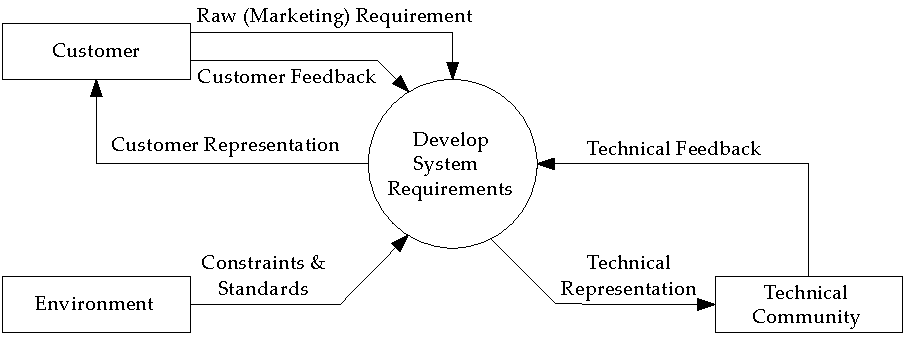
\includegraphics[width=4.6in,height=1.7in]{image1.pdf}
\caption{Requirements Specification development processes
from IEEE Std. 1233-1998. The three input sources to the process are the
customer, environment, and technical community.}
\label{figure: ieeeRequirements}
\end{figure}

\section{Engineering Requirements}
\label{section:engineering-requirements}

Before developing the complete Requirements Specification, designers
need to first determine individual engineering requirements.
\emph{\textbf{Engineering requirements}} are short statements that
address a technical need of the design. A simple example is ``\emph{The
system should be able to supply 50 watts of power.}'' This section
identifies the desirable properties of engineering requirements, methods
of identifying requirements, and provides numerous examples.

\subsection{Properties of an Engineering Requirement}
\label{section:properties-of-an-engineering-requirement}

Each engineering requirement should meet the four properties below
{[}IEEE Std. 1233-1998{]}:

\begin{enumerate}
\def\labelenumi{\arabic{enumi})}
\item
  \emph{Abstract.} This means that a given requirement should specify
  \emph{what} the system will do, not \emph{how} it will be implemented.
  This is the chicken and egg problem described earlier. It is
  frequently the most difficult property to satisfy since designers
  often have a preconceived concept for the solution. Unless absolutely
  necessary, the requirements should say nothing about the
  implementation. For example, a requirement stating that a certain
  microcontroller (i.e., technology) \ul{will} be used should be
  avoided. Admittedly, this is not always possible due to customer
  constraints or in cases where a system is being built upon
  pre-existing technology. A common analogy used for the ``\emph{what
  versus how}'' problem is that of designing a bridge. The requirement
  is to transport people from one side to other, without specifically
  stating the solution is a bridge, because another solution, like a
  ferry, may be a much more effective solution.
\item
  \emph{Verifiable.} Verifiability means that there should be a way to
  measure or demonstrate that the requirement is met in the final system
  realization. Doing so allows the system to be tested or verified
  against the requirements. The idea is that if there is no way to
  verify that the requirement is met, then it should not be a
  requirement. Verifiability is used to answer the question of
  ``\emph{Are we building the system correctly?}''
\item
  \emph{Unambiguous.} Each requirement should have a single unambiguous
  meaning and be stated with short complete sentences.
\item
  \emph{Traceable.} Requirements should be traceable marketing
  requirements. If the design doesn't satisfy the customer's needs, it
  won't be successful.
\end{enumerate}

Let's examine an example requirement for a robot whose objective is to
navigate autonomously within a specified environment. Consider the
following requirement

\begin{itquote}
The robot must have an average forward speed of 0.5 feet/sec, a top
speed of at least one foot/sec, and the ability to accelerate from
standstill to the average speed in under one second.
\end{itquote}

Are the four properties for an engineering requirement met? In terms of
the abstractness property, the answer is yes; it states what the system
must do, not how it will be implemented. In terms of the second
property, can the requirement be verified? Speed and acceleration are
directly testable in the final realization, and thus it is verifiable.
Is it unambiguous? It gives clear bounds for speed and acceleration.
Finally, traceability can't be shown without the marketing requirements
and is addressed later.

Now we analyze a second example requirement for the robot to see if it
meets the properties

\begin{itquote}
The robot must employ IR sensors to sense its external environment and
navigate autonomously with a battery life of one hour.
\end{itquote}

This requirement is not abstract since it identifies part of the
solution in terms of the sensor type and the fact that batteries must be
used. It is somewhat ambiguous in that it should specify what is meant
in terms of autonomous and the operating period. In terms of operating
period, should it work for exactly one hour and stop, or is greater than
an hour acceptable? Again, traceability can't be demonstrated without
the marketing requirements. This requirement would be hard to verify
without a good definition of what autonomous navigation in this context
means. A better requirement would be

\begin{itquote}
The robot must navigate autonomously, with the aid of only landmarks in
the specified environment, for a period of least one hour.
\end{itquote}

Realize that good requirements typically have two key elements in the
statement -- a description capability and condition. Capability
describes what the system must do and in the above requirement, that
capability is autonomous navigation. Conditions are measurable or
testable attributes of the capability and are critical for verification.


\subsection{A Fifth Property -- Realism}
\label{section:a-fifth-property-realism}

In addition to meeting the four properties, requirements should be
realistic or justified. This is not defined in the IEEE standard as a
property, but it is an important aspect that is often overlooked. To be
realistic, there should be a way of demonstrating that the target is
technically feasible. For example, a requirement could indicate that a
robot to should travel at a speed of 1,000,000 miles per hour, which
could be verifiable, unambiguous, and abstract -- yet, completely
unachievable. Realistic targets can be determined with a little
research, engineering know-how, creativity, or system modeling. One way
to do this is to assume a solution for the final system -- violating the
abstractness property. For example, consider the design of a robot where
some basic assumptions are made on the weight of the robot, the motors
used, the wheel size, and the battery selected. An engineering model
based upon these characteristics could be developed to predict
performance and estimate realistic requirements. Alternatively, target
requirements can be based upon an actual prototype, where a model or
experimental system is developed to show that a particular requirement
is feasible. This is how the technical community in 
Figure~\ref{figure: ieeeRequirements}
feeds into the requirements process.

The use of benchmarking to identify similar systems and their
performance provides a reference for realistic targets. It is generally
hard to surpass the performance of well-developed products and systems
on a first-generation design. An exception is with new and innovative
approaches that allow you to surpass the competition. Competitive
benchmarks may also be obtained from similar, but not necessarily
identical, products. Experience working with a particular technology or
previous generations of a system also provides guidance in selecting
realistic targets. That being said, organizations wishing to gain or
maintain a market edge often press the development team to achieve
performance on new generations that were once believed to be
unrealistic. Sometimes it just may not be feasible to determine the
technical feasibility of requirements. In such cases, the requirements
should have a certain amount of tolerance built into them and be updated
as development proceeds.

\subsection{Constraints}
\label{section:constraints}

One of the inputs to the requirements process in Figure~\ref{figure: ieeeRequirements}
is the environment, serving as the source of both constraints and standards. In
reality, all engineering requirements impose some sort of constraint on
a design, but in design a constraint is a special type of requirement. A
\emph{\textbf{constraint}} is a design decision imposed by the
environment or a stakeholder that impacts or limits the design.
Constraint requirements often violate the abstractness property. For
example, a constraint requirement is

\begin{itquote}
The system must use a PIC18F52 microcontroller to implement
processing functions.
\end{itquote}

This constraint requirement specifies how the system will be
implemented. This could be because the project sponsor has developed a
great deal of expertise using this particular microcontroller and does
not want to spend the development time learning a new platform. Note
that a number of other references define constraints to be synonymous
with non-functional requirements (usually indicated as items that are
not specifically functions). However, that terminology is avoided here
since it is not well defined nor universally accepted.

\subsection{Standards}
\label{section:standards}

\emph{\textbf{Standards}} are exactly what the name implies, a standard
or established way of doing things that ensure interoperability. Without
standards, the use of technology would be severely limited, if not
downright impossible. Standards ensure that products work together, from
home plumbing fixtures to the modules in a modern computer. Imagine if
every computer manufacturer had their own communication standard,
instead of following established protocols such as RS-232, TCP/IP, and
USB---computers would have a hard time printing, sending email, instant
messaging, or surfing the Internet! Furthermore, standards ensure the
health and safety of products that people use every day. Identifying and
following standards is an expected part of good engineering practice.

The focus in this chapter is on identifying standards that impact the
requirements and ultimately the design. The question becomes, what
standards are relevant to your project and how do you use them? There
are different levels of interaction with standards that we denote as:
user, implementation, and development levels. At the \emph{user level},
the standards are simply employed in the design, and detailed technical
knowledge of the standard is typically not necessary. For example, when
using a component that communicates to other devices, it is likely that
a standard communication protocol is used. Other than having to
configure software or hardware to communicate with the standard,
detailed knowledge of the standard isn't required. Another example would
be in developing software to display digital images in a standardized
format such as JPEG-2000 (Joint Photo Experts Group), in which case it
is likely that existing software components would be used to read and
display data in this format.

At the \emph{implementation level} details of the standard need to be
understood. Standards at the implementation level are most likely to
impact the design and the requirements. For example, when developing
low-level drivers for computer peripherals, you need to become an expert
on the underlying standard. Another example is reliability, where the
requirement may be that ``\emph{the system will have a reliability of
95\% in 10 years.}'' In this case a reliability standard, such as
\ul{Military Handbook for Reliability Prediction of Equipment}
{[}MIL-HDBK 217F{]} may be employed, and its usage requires an
understanding of both the reliability theory and the standard itself.

New standards are constantly being developed and existing ones modified,
leading to the final level of interaction at the \emph{development
level}. Depending upon the standard, engineers from different
organizations, professional societies, and corporations take part in the
standards setting process. Many participants in this process are trying
to gain a competitive advantage for their products and services.

It can be difficult to navigate the world of standards; they tend to be
highly detailed and limited parts of a standard may apply to a project.
In addition, many standards are costly to obtain, while some are freely
distributed. The following is advice for identifying and employing
standards. First, conduct research on applicable standards. Virtually
all standards organizations maintain websites that provide basic
information on their particular standards. The IEEE Xplore database is a
good place to start since it has a wide variety of standards and
provides free searchable abstracts. Many companies and universities have
subscriptions databases of complete standards. Second, determine the
expected level of interaction. Based upon your analysis of the problem,
do you foresee applying standards? Or will you need to develop an
in-depth knowledge at the implementation level? In the latter case, you
need to obtain detailed information on the applicable standards.
Finally, you should consider asking your client. They may have their own
internal standards and procedures to follow, and they may have experts
on the applicable standards.

The list below identifies some of the types of standards that may be
employed in a project and included in the requirements.

\begin{itemize}
\item
  \emph{Safety}. Safety standards address how to design for safety and
  how to test products to ensure that they are safe.
\item
  \emph{Testing}. Testing standards are often related to safety, but are
  broader in scope. For example, standardized benchmark tests are used
  for comparing computational performance, one well-known standard being
  the SPEC (Standard Performance Evaluation Corporation) benchmarks.
\item
  \emph{Reliability}. Reliability standards address general reliability
  principles and design methods for different classes of systems.
  Another practical aspect is in the estimation of reliability of
  electronic systems, such as the IEEE and military reliability
  standards.
\item
  \emph{Communications.} They address how electronic systems communicate
  and transfer information, such as in computing, telephony, and
  satellite communications.
\item
  \emph{Data Formats}. Standard data formats ensure that systems and
  software can properly share information. Examples include image,
  video, and database standards.
\item
  \emph{Documentation}. There are standards for technical report
  documentation. In addition, there are standards for documenting
  processes and business practices, a well-known case being the ISO
  (International Standards Organization) 9000 and subsequent standards.
\item
  \emph{Design Methods.} Certain design techniques are standardized as
  well. Examples include software design methodologies, and the use of
  design languages such as the Hardware Description Language (HDL) and
  the Unified Modeling Language (UML).
\item
  \emph{Programming Languages.} Programming language syntax is
  standardized so that software maintains a level of portability between
  systems and compilers.
\item
  \emph{Connector Standards.} Standards for cable connections are common
  and should be followed to ensure that systems are easily interfaced
  and manufactured.
\item
  \emph{Meta-Standards.} Some standards are a combination of multiple
  standards known as meta-standards. For example, the RS-232 standard is
  really a combination of a mechanical standard describing the connector
  physical dimensions connector, an electrical standard describing the
  voltages, a functional standard describing the pins and their
  function, and a procedural standard describing how entities
  communicate.
\end{itemize}

\subsection{Identifying Engineering Requirements}
\label{section:identifying-engineering-requirements}

There are many techniques for identifying requirements listed below
{[}IEEE Std. 1233-1998{]}:

\begin{itemize}
\item
  Structured workshops and brainstorming sessions.
\item
  Interviews, surveys, and questionnaires.
\item
  Observation of processes or devices in use.
\item
  Competitive benchmarking and market analysis.
\item
  Prototyping and simulations.
\item
  Research and technical documentation review.
\end{itemize}

Many requirements may be specified for a design, but knowing which to
include is the challenge. The remainder of this section is a guide to
describe the types of engineering requirements that may be specified for
electrical and computer systems. Requirements in categories of
performance and functionality are presented first as they are often
critical, followed by an alphabetical grouping of a potpourri of other
types requirements. \textbf{This taxonomy of requirements is by no means
definitive or inclusive of all possibilities, and the design team needs
to carefully determine those that are applicable to the particular
situation. Careful attention must be given to the verifiability of
requirements for the particular application.}

\subsection*{Performance}
\label{subsection:performance}

These requirements reflect a critical aspect of the performance of the
system or device. They often are characterized by time, accuracy,
throughput, or percentage error. The following is an example requirement
that might be used in a security application with camera surveillance.

\begin{itquote}
The system should detect 90\% of all human faces in an image.
\end{itquote}

In order to verify this, a test might be constructed where the system is
presented with a large database of face images that the system was not
developed or trained with. The number of faces correctly detected would
then be determined. Here is another example performance requirement for
a system that measure part location

\begin{itquote}
The system should be able to measure part location to within ± 1mm.
\end{itquote}

One way to verify this would be to take independent measurements of the
system's ability to measure part location and compare them to the result
of the system. The following is an example that could apply to software
response time.

\begin{itquote}
The system should retrieve the user data no less than three seconds for
90\% of requests and in a maximum of six seconds for all requests.
\end{itquote}

This could be verified by constructing a test where a large number of
queries for user data are presented to the software under a variety of
operating conditions and the response time measured. Yet another example
is:
\begin{itquote}
The system should be able to process video data at a rate of 30 frames
per second.
\end{itquote}

This could be verified by providing an input video stream at the frame
rate and testing to ensure that proper processing occurs. The test
procedure would need to specify length and number of videos to test,
issues that are addressed in Chapter 7. A final example of performance
is one that could apply to electrical audio amplification

\begin{itquote}
The amplifier will have total harmonic distortion of less than 1\%.
\end{itquote}

Total harmonic distortion is a measure that quantifies how closely an
amplifier is able to replicate the original signal. This would likely be
verified using laboratory instrumentation to measure the harmonic
distortion in the output signal.


\subsection*{Functionality}
\label{subsection:functionality}

These requirements describe the type of functions that a system should
perform. Often, they provide inputs, outputs, and the transformation
that the system will perform on the inputs. This is examined further in
Chapter 5, which presents functional design techniques. The following is
an example, where the input is ambient air temperature is converted to a
digital readout. It also has a performance aspect in that the accuracy
is specified.

\begin{itquote}
The system will convert ambient temperature to a digital readout of
temperature with an accuracy of 1\% over the measurement range.
\end{itquote}

The following is an example from a real capstone project to develop a
wireless mouse that is worn by the user and integrated into a glove.

\begin{itquote}
The system will implement the left and right button functions of a
standard mouse.
\end{itquote}

The following are several functional examples for software systems.

\begin{itquote}
The user shall be able to search all five company internal databases. \\ \\
The system will protect the user's identity with 128-bit encryption.
\end{itquote}

Note that in these last two cases, verification would be by inspection.


\subsection*{Economic}
\label{subsection:economic}

Economic requirements include the costs associated with the development
(design, production, maintenance) and sale of a system. They may also
include the economic impact of the final system, such as how it will to
contribute to profits or save the user money. Two example economic
requirements are below.

\begin{itquote}
The costs for developing the system (labor and parts) should not exceed
\$50,000. \\ \\
The total parts and manufacturing costs cannot exceed \$500 per unit.
\end{itquote}

\subsection*{Energy}
\label{subsection:energy}

Virtually all systems consume and/or produce energy and thus have energy
requirements. Energy consumption is the amount of power that a system
consumes, and may be specified in terms of maximum, minimum, or average
values. Example requirements are

\begin{itquote}
The system will have an average power consumption of 500mW. \\ \\
The system will have a peak current draw of 1A.
\end{itquote}

These requirements could be verified by measuring current and voltage
draws under the different operating conditions, or by estimating the
power drawn by all components in the system.


Operating lifetime addresses how long the system will operate from a
given power source. For battery-powered devices, operating time is
critical, and the lifetime for a given source may be an important
requirement. An example of such a requirement is

\begin{itquote}
The system will operate for a minimum of three hours without needing to
be recharged.
\end{itquote}

Source characteristics refer to the characteristics of the input and/or
output sources, such as voltage, current, impedance, frequency, number
of phases, and power requirements. An example requirement is

\begin{itquote}
The system will operate from a 12V source that supplies a maximum
current of 300mA.
\end{itquote}

\subsection*{Environmental}
\label{subsection:environmental}

These requirements address the impact of the design on the external
environment and usage of the earth's resources. For example, energy
usage is an important factor and example requirement is as follows

\begin{itquote}
The system will use 20\% less energy than the industry average for
similar products and qualify for US Energy Star certification.
\end{itquote}

Recyclability is the ability to dismantle a product into its constituent
materials for reuse in other products. European countries have
regulations on the recyclability of consumer products. In many cases,
the producer of a product is responsible for its safe disposal once its
service life is over. An example requirement is as follows

\begin{itquote}
50\% of the modular components will be able to be repaired and re-used
in similar products.
\end{itquote}

\subsection*{Health and Safety}
\label{subsection:health-and-safety}

The health and safety of anyone affected by the final product is an
especially important consideration. For example, IEEE and ANSI standards
provide guidance on safe levels for exposure to radio frequency electric
fields.

\begin{itquote}
The system will not expose humans to unhealthy levels of
electromagnetic radiation and will meet conditions for safe operation
identified in ANSI Std. C95.1.
\end{itquote}

There is a tendency to think that physical harm is not an issue in
electrical and computer systems, but many electronic systems control
mechanically moving parts. Consider the design of an automatic garage
door system. An example constraint could be that

\begin{itquote}
The door should stop moving if a person or object is detected in the
door path.
\end{itquote}

This could also translate into further engineering requirements on the
amount of force on the door required to trigger it to stop. There are
many safety standards, and two that are widely applied for consumer
products are the UL (Underwriters Laboratory) and CE (Common European)
standards. Examples are

\begin{itquote}
The system will use only UL approved components.\\ \\
The final system will be meet UL and CE standards and be tested at an
independent laboratory for approval.
\end{itquote}

\subsection*{Legal}
\label{subsection:legal}

Designs should not infringe upon existing patents, copyrights, and
trademarks, particularly if the intention is to sell the product. Patent
searches should be conducted, and search capabilities are available at
the United States Patent Office website
(\href{http://www.uspto.gov}{www.uspto.gov}). An example is

\begin{itquote}
An intellectual property search will be conducted to ensure that there
is no infringement on prior patents.\\ \\
This could be verified by having an external firm will conduct the
patent search and evaluate the design against existing intellectual
property.
\end{itquote}

Security and privacy constraints apply to systems that handle sensitive
data or personal communications. The ability of computing systems to
withstand malicious attacks by hackers is another consideration, and the
use of firewalls or other protective measures may be warranted. Examples
are

\begin{itquote}
The system will protect the user's identity with 128-bit encryption as
required by law.
\end{itquote}

\subsection*{Maintainability}
\label{section:maintainability}

The maintenance of the system being developed and compatibility with
other systems are often considerations. Will the system be designed so
that it can be reused in future applications? This is common in software
development where the objective is to design modules that are reliable
and flexible enough to be used in other applications. It is also a
consideration in terms of the reusability of electronic or digital
components in future system upgrades. An example reuse constraint is

\begin{itquote}
The software should maintain downward capability and be able to use
version 2 object libraries.
\end{itquote}

After a product goes into service, it enters the maintenance phase,
where it is maintained and upgraded. In software designs this is an
important consideration, as software is regularly upgraded and
maintained. On the hardware side, maintenance can be facilitated by the
use of plug-in modules that are easily removed and replaced. Examples
are

\begin{itquote}
The system will initially be available to 100 users at five field
locations, and within one year must be expanded to address usage by
5,000 users company-wide.\\ \\
The system should have a modular design such that failed components can
be replaced by a technician in under 15 minutes.
\end{itquote}

There may be internal restrictions on system development imposed by the
company based on their internal expertise and ability to maintain the
system, such as the following constraint requirement.

\begin{itquote}
The system will use only PIC microcontrollers.
\end{itquote}

\subsubsection*{Manufacturability}
\label{subsection:manufacturability}

A prevalent product development paradigm that used to be employed in
many engineering organizations was to ``\emph{throw the design over the
wall}.'' What this meant is that the design and development team would
create a new product and hand it off to the manufacturing team to
produce (throw it over the wall and run), often without having
considered the manufacturability of the product. The manufacturing team
would then address how to produce the design, and in many cases could
not do so without major redesign. Fortunately, this has given way to
much better concurrent engineering practices where all aspects of
product development are considered throughout the process. All of the
examples presented here are constraints, in that that they are external
decisions that limit the design.

Size is a consideration in terms of the amount of space the final design
will occupy, particularly if it has to be physically integrated with
other components. An example constraint requirement is

\begin{itquote}
The system must be manufactured on a circuit board with dimensions of no
greater than 1''x2''.
\end{itquote}

The realization and portability of the system is a consideration. For
example, with electronics, will it be built on a printed circuit board?
Following design rules and file format guidelines is important for
manufacturing printed circuit boards and integrated circuits. A chip
foundry may require that integrated circuit layouts utilize certain file
formats. Examples are below, which again are clear constraints on the
design.

\begin{itquote}
The system will be manufactured using three layer printed circuit board
technology.\\ \\
The product should be run on the Linux operating system.
\end{itquote}

The use of readily available parts, instead of low volume or hard to
find components, improves manufacturability, and an example is

\begin{itquote}
The design shall only incorporate components that can be purchased
through two of our main suppliers.
\end{itquote}

\subsubsection*{Operational}
\label{subsection:operational}

Operational requirements address the physical environment in which the
system will operate. Characteristics could be temperature, humidity,
electromagnetic radiation, shock, and vibration. Note, that these can
often be quite difficult to verify and may require specialized equipment
to do so. An example temperature operational requirement is

\begin{itquote}
The system should be able to operate in the temperature range of 0°C to
75°C.
\end{itquote}

This could be tested via test in an environmental chamber which the
operation of the system is tested over the complete temperature range.
Alternatively, indirect verification is a possibility. For example, in
the design, only components that are known to meet this operational
requirement, as specified in their product datasheet, could be used.


Depending upon the customer needs, the system may be tested in an
environmental chamber to verify that the requirement is met. Humidity is
similar in concept to the temperature requirement, addressing the
required ambient humidity range. A system may also need to be
water-resistant (withstand rain and snow) or waterproof (be submersible
in water). An example requirement is

\begin{itquote}
The system must be waterproof and operate while submersed in water.
\end{itquote}

Be careful with the differences between waterproof (submersible in
water) and water-resistant, which indicates the ability to withstand
outdoor elements such as rain and snow. For example, outdoor decorative
lights are water-resistant, but not waterproof.


Depending upon the environment, the system may need to withstand
vibrations. Bounds are typically specified in terms of frequency,
magnitude, and duration of the vibration. An example requirement is

\begin{itquote}
The system must be able to withstand vibrations of up to 60Hz with a
peak magnitude of 1mm for a period of 1 minute.
\end{itquote}

Electromagnetic Interference \emph{(EMI)} results from any
electromagnetic energy that interferes or disturbs the operation of an
electronic system. Electronic systems may produce electromagnetic
radiation and limits may need to be placed upon the amount of radiation
emitted. EMI is typically measured with specialized testing apparatus.
Conversely, a system may need to be able to operate properly given a
certain level of EMI.

The system may need to withstand a specified amount of shock and still
operate. This may be measured in G-force or via heuristics. An example
requirement is

\begin{itquote}
The system should withstand a drop from a height of six feet and still
operate.
\end{itquote}

\subsubsection*{Political}
\label{subsection:political}

Political constraints address relationships to political, governmental,
or union organizations. Examples include obtaining governmental
approvals, resolving trade barriers, and determining the acceptance of
systems for use in unionized environments. Examples are below.

\begin{itquote}
The system will need to obtain FDA approval before it can be sold to
medical users.\\ \\
The software will comply with the Digital Millennium Copyright Act.
\end{itquote}

\subsubsection*{Reliability and Availability}
\label{subsection:reliability-and-availability}

This refers to the expected period of time that a system will operate
properly. Measures of r\emph{eliability} include failure rates and mean
time to failure. Estimation of system reliability is given detailed
coverage in Chapter 8. The following is an example of a reliability
requirement.

\begin{itquote}
The system will have a reliability of 95\% in five years.
\end{itquote}

This requirement means that 95\% of the systems should be properly
operating (have not failed) in five years. Direct measurement of
reliability would not be possible, unless you are willing to wait five
years to see how many systems fail, thus the use of estimation. This
would require indirect verification using mathematical techniques to
estimate the system reliability.

\emph{Availability} is related to reliability, but addresses the amount
of time that a system is available for operation. Example availability
requirements are

\begin{itquote}
The system will be operational 99\% of the time.\\ \\
The system will be operational from 4AM to 10PM, 365 days a year.
\end{itquote}

These might be hard to verify this since it is only determined for sure
once the system is deployed. Verification would have to address under
which conditions the system would be tested to ensure this occurs.


\subsubsection*{Social and Cultural}
\label{subsection:social-and-cultural}

This addresses aspects such as benefits, risks, and acceptance of
products by the intended user or by society at large. For example,
robots have tremendous benefits for improving product quality, while
freeing people from dangerous and repetitive tasks. Yet when used in
automation, they present the risk of displacing workers and causing job
losses.

Many great products have fallen by the wayside because users were
unwilling to accept it. An example is the early Apple Newton Personal
Digital Assistant, the first product of its kind. The fatal flaw was
handwriting recognition that required a training process for accurate
recognition. This was not accepted by consumers and
Palm\textsuperscript{®} Computing solved the problem by employing a
simplified alphabet known as Graffiti. Graffiti was also seen as risky
when it was being developed, but due to its simplicity it was accepted
by consumers and the product became a huge success. In the mid 1980s,
Phillips electronics released the Laser Disk player, which failed
magnificently, but was far superior to VHS technology. Their failure was
attributed to the cost of the players and disks when compared to VHS.
Fifteen years later DVDs, with the help of computers, reached a price
point which now makes them preferable to VHS.

Will the system be used by engineers, technicians, laborers, doctors,
lawyers, or the general public? Each group has its own culture,
educational background, and willingness to accept innovations. Example
requirements are

\begin{itquote}
The product shall provide help menus to the user in either English or
Spanish. \\ \\
The software will be designed to easily be used by operators on the
manufacturing floor. The software will be tested by a group of 25
operators and the average time to learn the basic functionality of the
software will not exceed 8 hours.
\end{itquote}

\subsubsection*{Usability }
\label{subsection:usability}

\emph{Usability requirements} address the ease of use of a system.
Although they are quite common, they are often difficult to verify.
Usability can address how long it takes to learn the product and
satisfaction by the end-user or a group of users. To aid in verification
conditions can be placed on the number of menus in the system, an
estimated learning time, and number and types of errors the user is
allowed to make. An example requirement is that

\begin{itquote}
Users of the system should be able to learn 80\% of its functionality
within two hours.
\end{itquote}

The method of verification would need to be clearly specified, such as,
a group of 25 test users who have never used the product will be
provided two hours to learn the product. Another example of a usability
requirement is

\begin{itquote}
The system will have a maximum of 20 functions and a maximum of two
menus of depth.
\end{itquote}

\section{Developing the Requirements Specification}
\label{section:developing-the-requirements-specification}

The Requirements Specification is the complete set of all system
requirements. The steps in developing the Requirements Specification are
to:

\begin{itemize}
\item
  Identify requirements from the customer, environment, and the
  technical community (focus of the previous section).
\item
  Ensure the engineering requirements are well-formed (meet the
  properties).
\item
  Organize the requirements. Similar requirements should be presented
  together and relationships between engineering and marketing
  requirements identified. The collection of requirements should meet
  the properties identified in this section.
\item
  Validate the Requirements Specification -- which means all
  requirements are examined to ensure they meet the needs of the
  stakeholders.
\end{itemize}

\subsection{Properties of the Requirements Specification}
\label{subsection:properties-of-the-requirements-specification}

The desirable properties of the Requirements Specification are as
follows {[}IEEE Std.1233-1998{]}:

\begin{enumerate}
\def\labelenumi{\arabic{enumi})}
\item
  \emph{Normalized (orthogonal) set}. There should be no overlap or
  redundancy between engineering requirements. A mathematical analogy is
  that of orthogonal vectors. For example, the x and y axes of the
  two-dimensional Cartesian space are orthogonal vectors, meaning that
  the projection (dot product) of one vector onto the other is zero.
  Ideally, all requirements should be orthogonal with no redundancy.
\item
  \emph{Complete set.} A complete Requirements Specification addresses
  all of the needs of the end-user and also those needs required for
  system implementation. Failure to define a complete set results in
  \emph{\textbf{under-specificity}} where not all needs are met.
\item
  \emph{Consistent}. The engineering requirements should not be
  self-contradictory.
\item
  \emph{Bounded.} The scope of the Requirements Specification should be
  identified. Determine the minimum acceptable bound for target values;
  going beyond what is necessary limits the design space of potential
  solutions. Applying unnecessary bounds results in
  \emph{\textbf{over-specificity}}.
\item
  \emph{Modifiable.} Requirements are typically considered to be
  evolutionary. This is because there are many unknowns at the start of
  a project, hence estimates for the requirements are made. The original
  requirements are known as \emph{\textbf{baseline requirements}}. The
  estimates can change as development proceeds, as long as the changes
  are communicated to and agreed upon by all affected parties. Versions
  of the requirements should be tracked and identified as modifications
  take place.
\end{enumerate}

\subsection{Requirements Validation}
\label{subsection:requirements-validation}

An important property of an engineering requirement that we saw earlier
was verifiability. Verifiability seeks to answer the question of whether
or not the system is being developed correctly, or \emph{``Are we
building the product correctly?''} A related concept is that of
validation, which seeks to answer the question ``\emph{Are we building
the correct product?}'' More formally, \emph{\textbf{validation}} is the
process of determining whether the system meets the needs of the
user---is it valid? This is more general in scope than verification and
more difficult to show. Requirements validation is usually carried out
by reviews of the requirements by a team of people. Validation is
demonstrated by being able to answer the following questions in the
affirmative {[}Som01{]}:

\begin{itemize}
\item
  For each individual engineering requirement, are the traceability and
  verifiability properties met? Is each requirement realistic and
  technically feasible?
\item
  For the Requirements Specification, are the properties of
  orthogonality, completeness, and consistency met?
\end{itemize}

  A complete Requirements Specification includes all the requirements,
  both marketing and engineering, along with the relationships between
  them. The relationships between the engineering and marketing
  requirements need to be described to ensure that all the marketing
  requirements are being addressed by design. The relationship between
  the marketing and engineering requirements is called a mapping
  because, like a mathematical mapping, it defines which elements of the
  domain (marketing requirements) are associated with which elements of
  the range (engineering requirements).


\section{Requirements Case Studies}
\label{section:requirements-case-studies}

This section presents case study examples of Requirements Specification,
most of which are from real capstone design projects. They are presented
in a table format that presents each engineering requirement, the mapped
marketing requirements (supporting the traceability property), and the
justification for each requirement. The marketing requirements are
summarized at the end of the table.

\subsection{Case Study: Car Audio Amplifier}
\label{subsection:case-study-car-audio-amplifier}

Table~\ref{table:audioRequireSpec} presents the Requirements Specification for a car audio
amplifier. This simple example was selected because of the relative ease
of understanding, broad familiarity with this type of device, and it
will be expanded upon later.

\begin{table}
\centering
\caption{Requirements Specification for an audio amplifier for
use in an automobile.}
\label{table:audioRequireSpec}
\begin{tabular}{ |p{2cm}|p{5cm}|p{5cm}|} 
\hline
\rowcolor{Gray}
\textbf{Marketing Requirements} & \textbf{Engineering Requirements} & \textbf{Justification} \\ \hline
                           
1, 2, 4 &
1.  The \emph{total harmonic distortion} should be \textless0.1\%. &
Based upon competitive benchmarking and existing
amplifier technology. Class A, B, and AB amplifiers are able to obtain
this level of THD. \\ \hline

1--4 & 
2.   Should be able to sustain an \emph{output power} that averages $\ge 35$
  watts with a peak value of $\ge 70$ watts. & 
This power range provides more than adequate sound
throughout the automobile compartment. It is a sustainable output power
for projected amplifier complexity. \\ \hline

2, 4 & 
3. Should have an efficiency $\eta > 40\%$. &
Achievable with several different classes of power amplifiers. \\ \hline

3 & 
4.   \emph{Average installation time} for the power and audio connections
  should not exceed 5 minutes. &
Past trials using standard audio and power jacks
demonstrate that this is a reasonable installation time. \\ \hline

1--4 & 
5.  The \emph{dimensions} should not exceed 6'' x 8''x 3''. &
Fits under a typical car seat. Prior models and
estimates show that all components should fit within this package
size. \\ \hline

1--4 & 
6.  \emph{Production cost} should not exceed \$100. &
This is based upon competitive market analysis and previous system designs. \\ \hline

\multicolumn{3}{|p{12cm}|}{
\textbf{Marketing Requirements}\newline
1.  The system should have excellent sound quality.\newline
2.  The system should have high output power.\newline
3.  The system should be easy to install.\newline
4.   The system should have low cost.
} \\ \hline
\end{tabular}
\end{table}

Audio power amplifiers are widely available devices, so the requirements
were determined through competitive benchmarks and knowledge of
amplifier circuit designs. The first engineering requirement directly
impacts sound quality and is known as total harmonic distortion (THD).
THD measures how closely the amplifier output signal follows the input
signal. It is desirable for an amplifier to have a linear relation
between input and output, where the output signal is identical to the
input signal, except for an amplification factor. In reality, all
amplifiers have some degree of nonlinearity or distortion. It is
measured by applying a pure sinusoid as the input to the amplifier,
which in the case of a perfectly linear amplifier produces a pure output
sinusoid of the same frequency. Any nonlinearity introduces unwanted
harmonic frequencies. THD represents the power of unwanted harmonics
relative to the power of the fundamental sinusoid. THD is typically less
than 1\% for a good amplifier.

The second requirement, output power, is quantified in terms of both
average and maximum values to minimize ambiguity. The third engineering
requirement addresses the efficiency of the power transfer, or how much
of the power consumed by the device is actually converted to audio
power. The fourth engineering requirement, ease of installation, is
perhaps easy to understand intuitively, and the expected installation
time provides the condition for verification. The fifth requirement
addresses the physical size of the device, and is important as it will
need to be installed somewhere in the vehicle.

\subsection{Case Study: iPod\textsuperscript{TM} Hands-Free Device}
\label{subsection:case-study-ipodtm-hands-free-device}

Table~\ref{table:ipod} presents the Requirements Specification for a hands-free
device whose intent is to allow a driver to communicate with an
iPod\textsuperscript{TM} audio player while driving. The Problem
Statement was presented in Chapter 2 (Section 2.6).

\begin{table}
\centering
\caption{Requirements Specification for the
iPod\textsuperscript{TM} Hands-Free Device.}
\label{table:ipod}

\begin{tabular}{ |p{2cm}|p{5cm}|p{5cm}|} 
\hline
\rowcolor{Gray}
\textbf{Marketing Requirements} & \textbf{Engineering Requirements} & \textbf{Justification} \\ \hline

4, 6 & 
1.  System will i\emph{mplement nine voice command} functions ( menu,
  play/pause, previous, next, up, down, left, right and select) and
  respond appropriately according to each command. &
  hese are the basic nine commands that are used to
control an iPod and will provide all functionality needed. \\ \hline

1, 3, 4, 7 & 
2.   The \emph{time to respond} to voice commands and provide audio
  feedback should not exceed 3 seconds. &
The system needs to provide convenient use by
responding to the user inputs within a short time period. Based on
research it was determined that the response time for the iPod is less
than 1 second and an average voice recognition system requires 2 seconds
to recognize commands. \\ \hline

4, 6 & 
3.   The \emph{accuracy} of the system in accepting voice commands will be
  between 95\% and 98\%. &
Research demonstrates that this is a typical accuracy
of voice recognition chips. Speaker independent systems can achieve 95\%
and speaker-dependent up to 98\%. \\ \hline

5, 6 & 
4.   The system should be able to \emph{operate} from a 12 V source and
  will draw a maximum of 150 mA. &
The automobile provides 12V DC. A current draw budget
estimate was developed with potential components and 150mA was an upper
limit of current estimated. \\ \hline

5, 6, 7 & 
5.  The \emph{dimensions} of the prototype should not exceed 6'' x 4'' x  1.5''. &
This system must be able to fit in a car compartment,
somewhere between the seats. Estimate is based upon a size budget
calculation using typical parts. \\ \hline

\multicolumn{3}{|p{12cm}|}{
\textbf{Marketing Requirements}\newline
1. Should not minimize or slow down the functional quality of the iPod.\newline
2.  User should be able to search for songs and artists and receive feedback on selection.\newline
3.  System should provide clear understandable speech.\newline
4.  System should be able to understand voice commands from user.\newline
5.  Should be able to fit and operate in an automobile.\newline
6.  Should be easy to use.\newline
7.  Should be portable.
} \\ \hline
\end{tabular}
\end{table}

To develop the marketing requirements, this team conducted an informal
survey of students on campus, asking the target group what their desires
for such a system would be. The first three engineering requirements are
related to the important issues of the system functionality and
performance. In order to develop justifications for some of the
requirements a prototype solution had to considered, although the
solution has not been formally posed. For example, in order to estimate
a time for responding to a user's command, some assumptions were made on
the types of components that might be used in the design. The last two
requirements are operational requirements, ensuring that the device will
work in its intended environment.

\subsection{Case Study: Gigabit Ethernet Card Testing}
\label{subsection:case-study-gigabit-ethernet-card-testing}

Table~\ref{table:gigabit} presents an example Requirements Specification developed for
the design of an experimental test setup {[}Ese03{]}. The Problem
Statement for this example was presented in Chapter 2, where the
objective was to design a system to test a gigabit Ethernet card for use
in a harsh operating environment. In particular, the effects of
temperature and vibration variations on the optical power margin, both
of which impact the bit-error rate and the system performance, were
determined.

\begin{table}
\centering
\caption{System Requirements for a Gigabit Ethernet card
testing project.}
\label{table:gigabit}

\begin{tabular}{ |p{2cm}|p{5cm}|p{5cm}|} 
\hline
\rowcolor{Gray}
\textbf{Marketing Requirements} & \textbf{Engineering Requirements} & \textbf{Justification} \\ \hline

1 & Must be able to measure the \emph{optical power output} with an
\emph{accuracy} of ± 0.5dB. & This is based upon commercially available
optical power measurement instruments. \\ \hline
2 & Must be able to measure the \emph{optical power output} from 10°C to
55°C. & This range simulates the operating environment, and 55°C is the
maximum operating temperature of the card. \\ \hline
2 & The system must maintain \emph{temperature accuracy} to within ± 1°C
during all tests. & Based upon accuracy of commercially available test
chambers. \\ \hline
3 & Must be able to measure optical power over a \emph{frequency range}
from 4Hz to 33Hz in increments of 1Hz. & The frequencies encountered in
actual operation will not exceed this range. \\ \hline
3 & The \emph{peak vibration amplitude} should be 0.01 inches. & The
amplitude in the operating environment will not exceed this value. \\ \hline
3 & The card should be tested at a given frequency for a \emph{duration}
of 1 minute. & This exceeds the expected duration of vibration at given
frequency that the system will encounter. \\ \hline
3 & The vibration effects should be tested in x, y, and z
\emph{directions}. & The system will encounter vibrations in multiple
directions. This will provide data on differences in directional
variation due to vibration. \\ \hline
3 & The experiment should determine \emph{resonant frequency} to an
accuracy of ± 0.5Hz. & This will provide data on worst case vibration at
the resonant frequency. \\ \hline

\multicolumn{3}{|p{12cm}|}{
\textbf{Marketing Requirements} \newline
1.  The measurement of the optical power should be accurate.\newline
2.  It should measure the effects of temperature variations on optical power.\newline
3.  It should measure effects of vibration on the fiber optic connector
  and optical power output.}  \\ \hline
\end{tabular}
\end{table}

The marketing requirements were quite brief and direct, and not
surprising due to the fact the customer in this case was group of
engineers who had a good idea of what they wanted. The engineering
requirements were selected based upon characteristics of the operating
environment, through discussion with the engineers, and via some
educated guesswork. Let's consider some of the requirements, starting
with the effects of temperature variation on the optical power output.
The testing requirement on the temperature range was selected based on
the operating environment, while the accuracy is driven by the test
equipment. The requirements also address the vibration testing
requirements, including the vibration frequency range, amplitude, and
resonant frequency.

\subsection{Case Study: Portable Aerial Surveillance System}
\label{subsection:case-study-portable-aerial-surveillance-system}

The Requirements Specification for the Portable Aerial Surveillance
System (Problem Statement presented in Chapter 2) is shown in Table~\ref{table:portableAerial}.
This system is intended to provide police and emergency responders with
a low-cost easy to deploy aerial surveillance system.

\begin{table}
\centering
\caption{System Requirements for the Portable Aerial
Surveillance System.}
\label{table:portableAerial}

\begin{tabular}{ |p{2cm}|p{5cm}|p{5cm}|} 
\hline
\rowcolor{Gray}
\textbf{Marketing Requirements} & \textbf{Engineering Requirements} & \textbf{Justification} \\ \hline

6 & 
 System will provide visual recognition of license plate text from a
  minimum distance of 150 feet during daytime and nighttime use. &
   Recorded images and video will be used as trial
evidence. The device's maximum height is 150 feet, so
the device should allow text recognition at an absolute minimum of that
distance. The device must be also usable during nighttime.\\ \hline

4, 9 & 
   The device must be operable by a single person. &
 A police officer dispatched alone in his or her cruiser
should be able to launch and operate the device with no assistance. \\ \hline

2 & 
 This device must remain airborne for a minimum of two hours. &
Based upon interviews with law enforcement users. This
is a time period that covers most emergency situations. \\ \hline

7, 8 & 
 The device will be able to be used in at least 14 mph winds.&
 Device will be used outdoors and in non-ideal
conditions in Erie, PA, where there is a 95\% chance that winds will be
at or below 14 mph. \\ \hline

7 & 
  The device must not exceed a height of 150 feet above ground level
  when in use. &
  This device must comply with FAA regulation 101.15 \\ \hline
  
3 & 

  Must fit into the trunk of a police cruiser. The Chevrolet Impala has
  a trunk measuring 54 inches wide by 38 inches deep by 16 inches high. &
 Will be transported in a police cruiser and must fit
into the trunk of the vehicle. \\ \hline

1 & 
  The device will cost less than \$3000 per year to operate. &
 The budget allotted to Erie county police departments
was \$16.7 million. 0.85\% of Erie\textquotesingle s annual budget would
allow for \$140,280 to be used for a helicopter. A device having less
than 2\% of the annual operating costs of a helicopter, and having many
of the same surveillance capabilities would be considered a reasonable
expense. \\ \hline

\multicolumn{3}{|p{12cm}|}{
\textbf{Marketing Requirements}\newline
1.  The device should be able to be held stationary in the air, meaning
  providing enough stability to provide functionality.\newline
2.  Should be capable of being deployed for a long period of time.\newline
3.   Should be able to be deployed by one person in 3-5 minutes.\newline
4.  Should record video with enough quality to be used as evidence.\newline
5.  Should be useful at night.\newline
6.  Should fit in the trunk of a car and withstand the stresses of
  transportation.\newline
7.  Should be repairable and reusable.\newline
8.  Should require minimal training to be operated by one person.\newline
9.  Should be relatively inexpensive compared to that of a helicopter.\newline
10.  Should be able to operate at an altitude above most buildings.\newline
11.  Should meet any applicable governmental regulations (such as FAA).\newline
12.  Should be able to operate in typical winter conditions.}  \\ \hline
\end{tabular}
\end{table}

This project was developed in conjunction with Penn State Behrend and
the Mercyhurst College's Institute for Intelligence Studies to meet a
need that the institute identified. The student team met with a number
of law enforcement officials to determine the needs. The first
engineering requirement addresses the critical functionality that the
system is to provide, while engineering requirements 2--5 address the
performance and ability to work in the outdoor environment. Note the
inclusion of a federal standard that drives the requirement on the
maximum deployment height of the device. Requirement 7 addresses the
cost, which can often be difficult to justify in student projects, but
in this case the team has developed a clear justification.

\section{Advanced Requirements Analysis}
\label{section:advanced-requirements-analysis}

This section examines more advanced methods that are used to analyze and
refine requirements. There are tradeoffs between the different
requirements and understanding them is valuable for refining the
requirements themselves and developing solution concepts. This section
addresses tradeoffs between engineering and marketing requirements,
tradeoffs between engineering requirements themselves, and benchmarking.
At the conclusion, all of this is integrated in to the well-known House
of Quality.

\subsection{The Engineering-Marketing Tradeoff Matrix}
\label{subsection:the-engineering-marketing-tradeoff-matrix}

This matrix identifies how engineering and marketing requirements impact
each other. To demonstrate its construction, we continue to examine the
automobile audio amplifier example from Table~\ref{table:audioRequireSpec}. 
The tradeoff matrix
is shown in Table~\ref{table:engMarketingMatrix}, where the marketing 
requirements constitute the
row headings and the engineering requirements the column headings.

\begin{table}
\centering
\caption{Engineering-marketing tradeoff matrix for the audio
amplifier. ↑=positive correlation, ↑↑=strong positive correlation,
↓=negative correlation, ↓↓=strong negative correlation.}
\label{table:engMarketingMatrix}

\begin{tabular}{|l|l|l|l|l|l|l|l|} 
\hline
\rowcolor{Gray}
  &   & \rotatebox[origin=c]{90}{THD} & 
  			\rotatebox[origin=c]{90}{Output Power} & 
  			\rotatebox[origin=c]{90}{$\eta$, Efficiency} & 
  			\rotatebox[origin=c]{90}{Install Time} & 
  			\rotatebox[origin=c]{90}{Dimensions} & 
  			\rotatebox[origin=c]{90}{Cost} \\ \hline
  
  \rowcolor{Gray}
  &   &  -      &  +                     & +               & -                   & -                    &  - \\ \hline

1) Sound Quality & + & ↑↑ & ↓ & & & ↓↓ & ↓↓ \\ \hline
2) High Power & + & ↓ & ↑↑ & ↑ & & ↓↓ & ↓ \\ \hline
3) Install Ease & + & & ↓ & & ↑↑ & ↑ & ↓ \\ \hline
4) Cost & - & ↓↓ & ↓ & ↓ & & ↓ & ↑↑ \\ \hline
\end{tabular}
\end{table}

One of the first things to note is that each requirement has an
associated polarity. A requirement with a positive/negative polarity,
denoted with a +/- symbol, means that increasing/decreasing that
requirement increases the desirability of the product, respectively. A
goal is considered a requirement with its polarity. For example, cost
almost universally has a negative polarity because decreasing cost
almost always makes a product more desirable.

The entries in the body of the matrix can be thought of as a correlation
that measures the ability to achieve the marketing and engineering goals
simultaneously. A positive correlation (↑) means that both goals can be
simultaneously improved, while a negative correlation (↓) means that
improving one will compromise the other. Not all correlations are of
equal importance, the strength of the correlation being denoted by the
number of arrows. Blanks entries in the matrix mean that there is no
correlation between the requirements.

To better understand the matrix, consider the entries in the top row
associated with sound quality. The relationship between THD and sound
quality is denoted by the double positive arrow. This relationship is
interpreted as

\begin{itquote}
The goal is to increase sound quality and decrease THD. There is a
strong positive correlation between them since decreasing THD increases
sound quality.
\end{itquote}

What wasn't so clear in the 1-to-1 mapping is that there is a link
between the goal of maximizing output power and the goal of maximizing
sound quality (second entry in the top row). This entry is interpreted
as

\begin{itquote}
The goal is to increase sound quality, to increase output power, and
there is negative correlation between them since increasing output power
will decrease sound quality.
\end{itquote}

That is because electronics can be designed to achieve larger output
power at the expense of sound quality. However, it gets a little more
complicated, since output power can be increased without loss in sound
quality, if more amplifier stages are employed. That increases the
dimensions and cost, thus the relationships between sound quality, cost,
and dimensions are identified in the first row. When creating the
entries in the matrix, it should be assumed that only the associated
requirements can vary and that all others are held constant. When
finished, the matrix allows a quick and easy reading of the tradeoffs
between engineering and marketing requirements. This example
demonstrates the complex nature of a seemingly simple device, and
provides a much clearer picture of the design tradeoffs involved.

\subsection{The Engineering Tradeoff Matrix}
\label{subsection:the-engineering-tradeoff-matrix}

The example of output power in the previous section illustrates the need
to examine the tradeoffs between the engineering requirements, which are
shown in Table~\ref{table:engTradeOff}. In this table the engineering requirements
constitute the headings for both the row and column entries. Only the
entries above the upper diagonal elements are filled in due to the
redundancy of the lower diagonal elements. Again, positive and negative
correlations are indicated along with the strength of correlation.

Let's examine the tradeoffs involved with output power. High output
power can be achieved at the expense of THD as shown in the first row of
the table. The second row indicates that there is a positive correlation
between efficiency and output power, since the more efficient an
amplifier is, the more power it can deliver. There is a negative
correlation between the dimensions and power, since larger parts and
greater surface area aid in dissipating more power. Finally, there is a
negative correlation between the output power and cost because of the
greater size and number of parts needed to achieve higher power.

\begin{table}
\centering
\caption{The engineering tradeoff matrix for the audio
amplifier. ↑=positive correlation, ↓=negative correlation.}
\label{table:engTradeOff}

\begin{tabular}{ |l|l|l|l|l|l|l|l|} 
\hline
\rowcolor{Gray}
      &   & \rotatebox[origin=c]{90}{THD} & 
  			\rotatebox[origin=c]{90}{Output Power} & 
  			\rotatebox[origin=c]{90}{$\eta$, Efficiency} & 
  			\rotatebox[origin=c]{90}{Install Time} & 
  			\rotatebox[origin=c]{90}{Dimensions} & 
  			\rotatebox[origin=c]{90}{Cost} \\ \hline
  
 \rowcolor{Gray}
  &   &  -      &  +                     & +               & -                   & -                    &  - \\ \hline
THD 			& - 		& \cellcolor{blue!25}& ↓ & & & ↓ & ↓ \\ \hline
Output Power 	& + 	& \cellcolor{blue!25}& \cellcolor{blue!25}& ↑ & & ↓ & ↓ \\ \hline
$\eta$, Efficiency 		& + 	& \cellcolor{blue!25}& \cellcolor{blue!25}& \cellcolor{blue!25}& & ↑ & ↓ \\ \hline
Install Time		& - 		& \cellcolor{blue!25}& \cellcolor{blue!25}& \cellcolor{blue!25}& \cellcolor{blue!25}& ↓ & \\ \hline
Dimensions 		& - 		& \cellcolor{blue!25}& \cellcolor{blue!25}&\cellcolor{blue!25} & \cellcolor{blue!25}& \cellcolor{blue!25}& ↓ \\ \hline
Cost 			& - 		& \cellcolor{blue!25}& \cellcolor{blue!25}& \cellcolor{blue!25}& \cellcolor{blue!25}& \cellcolor{blue!25}& \cellcolor{blue!25} \\ \hline
\end{tabular}
\end{table}

\subsection{Competitive Benchmarks}
\label{subsection:competitive-benchmarks}

Competitive benchmarking helps to select targets for the engineering
requirements. By analyzing competing systems, a better understanding is
gained of what is realistic and where the design may potentially
outperform the competition. The benchmark table lists the requirements
in the row headings and the competitors in the column headings as shown
in Table~\ref{table:benchmarkAudio}.

\begin{table}
\centering
\caption{Competitive benchmarks for the audio amplifier.}
\label{table:benchmarkAudio}
\begin{tabular}{ |> {\columncolor{Gray}} c  |l|l|l|} 
\hline
\rowcolor{Gray}
  & \textbf{Apex Audio} & \textbf{Monster Amps} & \textbf{Our Design}\\ \hline
\textbf{THD} & 0.05\% & 0.15\% & 0.1\% \\ \hline
\textbf{Power} & 30W & 50W & 35W \\ \hline
\textbf{Efficiency} & 70\% & 30\% & 40\% \\ \hline
\textbf{Cost} & \$250 & \$120 & \$100 \\ \hline
\end{tabular}
\end{table}

\subsection{The House of Quality}
\label{subsection:the-house-of-quality}

A well-known tool for developing requirements is the House of Quality
(HOQ). The HOQ is part of a product development process known as Quality
Functional Deployment (QFD) that is widely used in industry. QFD is a
series of processes for product development that incorporate the needs
of the customer throughout the system lifecycle. It encompasses design,
manufacturing, sales, and marketing. QFD is characterized by a series of
matrices that have a visual appearance similar to that of a house. The
matrices relate different aspects of the development process and are
effective for communicating between different units in an organization.
There are houses for different phases of product development, but here
the focus is on using the HOQ for the Requirements Specification. A HOQ
for the audio amplifier example is shown in Figure~\ref{figure:houseOfQuality}. 
It contains all
of the elements that we have addressed so far---marketing requirements,
engineering requirements, engineering-marketing tradeoffs, engineering
tradeoffs, and the target values for the engineering requirements. The
HOQ is presented for completeness, but is redundant since it contains
all of the information already presented in Tables \ref{table:engMarketingMatrix}--\ref{table:benchmarkAudio}. The HOQ
also becomes visually overwhelming and hard to read as problem
complexity grows.


\begin{figure}
\centering
\caption{The complete House of Quality for the audio
amplifier example. This integrates the information in Tables 
\ref{table:engMarketingMatrix}, \ref{table:engTradeOff}, and \ref{table:benchmarkAudio}.}
\label{figure:houseOfQuality}

\begin{tabular}{ |p{5cm}|l|l|l|l|l|l|l|} 
\hline
\rowcolor{Gray}
      &   & \rotatebox[origin=c]{90}{THD} & 
  			\rotatebox[origin=c]{90}{Output Power} & 
  			\rotatebox[origin=c]{90}{$\eta$, Efficiency} & 
  			\rotatebox[origin=c]{90}{Install Time} & 
  			\rotatebox[origin=c]{90}{Dimensions} & 
  			\rotatebox[origin=c]{90}{Cost} \\ \hline
 \rowcolor{Gray}
  &   &  -      &  +                     & +               & -                   & -                    &  - \\ \hline
1) Sound Quality & + & ↑↑ & ↓ & & & ↓↓ & ↓↓ \\ \hline
2) High Power & + & ↓ & ↑ & ↑↑ & & ↓↓ & ↓ \\ \hline
3) Install Ease & + & & ↓ & & ↑↑ & ↑ & ↓ \\ \hline
4) Cost & - & ↓↓ & ↓ & ↓ & & ↓ & ↑↑ \\ \hline
\multicolumn{2}{|c|}{\textbf{Targets for Engineering Requirements}} &
		\rotatebox[origin=c]{90}{\textless0.1\%} &
		\rotatebox[origin=c]{90}{35 Watts} &
		\rotatebox[origin=c]{90}{\textgreater{} 40\%} &
		\rotatebox[origin=c]{90}{$\leq 5$ minutes} &
		\rotatebox[origin=c]{90}{6 x 8 x 3 inches} &
		\rotatebox[origin=c]{90}{$\leq \$100$} \\  \hline
\end{tabular}
\end{figure}

\section{Project Application: The Requirement Specification}
\label{section:project-application-the-requirements-specification}

The following is a recommended format for a Requirements document that
integrates the Problem Statement from Chapter 2.

\begin{itemize}
\item
  \emph{Needs, Objectives, and Background.} Include the elements from
  the Problem Statement in Chapter 2.
\item
  \emph{Requirements}. Identify the marketing requirements, engineering
  requirements, and justification in a table format (see Tables~\ref{table:audioRequireSpec} --
  \ref{table:portableAerial}). Supplement this with tradeoff matrices and competitive
  benchmarks as necessary.
\end{itemize}

Table~\ref{table:benchmarkAudio} presents a self-assessment checklist for the Requirements
 Specification.
  
\begin{table}
\centering
\caption{Self-assessment checklist for the Requirements
Specification. 1 = Strongly Disagree, 2 = Disagree, 3 = Neutral, 4 =
Agree, 5 = Strongly Agree.}

\label{table:requirementsCheckList}
\begin{tabular}{ |p{10cm}|l|} 
\hline
\rowcolor{Gray}
\textbf{Engineering Requirements} & \textbf{Score}\\ \hline
Each engineering requirement is abstract. & \\ \hline
Each engineering requirement is verifiable. & \\ \hline
Each engineering requirement is unambiguous and written as a concise
statement. & \\ \hline
Each engineering requirement can be traced to a user need. & \\ \hline
Each engineering requirement is realistic and has a justification
provided. & \\ \hline
Standards and constraints applicable to the project have been identified
and included. & \\ \hline

\rowcolor{Gray}
\textbf{The Requirements Specification} & \\ \hline
The requirements are normalized, with minimal redundancy and overlap.
& \\ \hline
The engineering requirements are organized by similarity. & \\ \hline
The requirements are complete, addressing all needs. & \\ \hline
The requirements are bounded (not over-specified). & \\ \hline
The requirements have been validated and agreed upon by all
stakeholders. & \\ \hline
\end{tabular}
\end{table}

\section{Summary and Further Reading }
\label{section:summary-and-further-reading}

This chapter presented a process for developing the Requirements
Specification, which consists of identifying the requirements from the
user, environment, and input of the technical community. The desirable
properties of engineering requirements and the complete Requirements
Specification were presented. The verification of a requirement is
particularly important, as it seeks to help in answering if the system
is being built correctly. Requirements validation addresses whether the
requirements meet the needs of the user, or if the correct product is
being designed. Tools for benchmarking and analyzing the tradeoffs
between requirements were given. Proper determination of the
requirements significantly influences all subsequent phases of the
design, thus the final requirements document should be agreed upon by
all stakeholders.

The processes presented here were developed from research in the field
and the authors' teaching experiences. Pugh {[}Pug90{]} presents a good
perspective on identifying requirements and constraints, although with
more emphasis on mechanical systems. The article by Robert Abler
{[}Abl91{]} is a short primer that provides good advice on how to
develop specifications that overlaps with the properties presented in
the IEEE Standard 1233 {[}IEEE Std. 1233-1998{]}.

The HOQ technique was originally developed by Hauser and Clausing
{[}Hau88{]} and has gained wide acceptance. Their original article
provides a case study of the technique applied to the design of
automobile door seals as implemented by Toyota Motor Corporation.
Ullrich and Eppinger {[}Ull03{]} present a good perspective on
developing specifications employing the QFD techniques and the HOQ with
an emphasis on the voice of the customer.

\section{Problems}
\label{section:reqSpecProblems}
\graphicspath{ {./chapter03/FigSolutions} }

\begin{enumerate}
\def\labelenumi{\arabic{enumi}.}
\item
  Briefly describe the four properties of an engineering requirement.
  
  
\item
  Identify the three levels of standards usage and what is meant by each one.
  
 \begin{onlysolution}
 \textbf{[R]}
 \itshape
  The three levels of standards usage are user, implementation, and
development. The \textbf{user level} simply incorporates the standard
within the design without the need for technical knowledge concerning
the standard. However, the \textbf{implementation level} requires an
in-depth knowledge of the standard -- developing hardware drivers and
ensuring reliability requirements. As with the implementation level, the
\textbf{development level} also requires knowledge of the standard in
order to further develop and modify its predecessor.
\end{onlysolution}
  
  
\item
  For each of the engineering requirements below, determine if it meets
  the properties of abstractness, unambiguous, verifiable, and
  realistic. If a requirement does not satisfy the properties, restate
  it so that it does:


\begin{enumerate}
\def\labelenumi{\alph{enumi})}
\item
  The TV remote control will be easy to use.
  
\begin{onlysolution}
\textbf{[A]}
 \itshape
 Abstractness: \textbf{Yes} -- doesn't give details on implementation\\
Unambiguous: \textbf{Maybe} -- there is not a clear definition of
easy-to-use. It could be possible to develop some metrics for easy to
use, such as size of buttons, number of buttons, etc.\\
Verifiable: \textbf{Maybe -} this relates back to the ambiguity of
easy-to-use. If the easy-to-use property is defined, then it could be
verifiable.
\end{onlysolution}
  
  
\item
  The robot will identify objects in its path using ultrasonic sensors.
  
\begin{onlysolution}
\textbf{[A]}
 \itshape
Abstractness: \textbf{No} -- provides a solution to the problem (ultrasonic sensors)\\
Unambiguous: \textbf{No} -- it will identify objects in its path, is
somewhat clear. However, could be better defined if its path were
defined, as well as the distance of detection\\
Verifiable: \textbf{No} (Because it is not unambiguous.)\\
\textbf{Restatement:} ``The robot will identify objects in its forward
path within 3 feet of the robot.''
\end{onlysolution}

\item
  The car audio amplifier will be encased in aluminum and will operate
  in the automobile environment.
  
  \begin{onlysolution}
  \textbf{[A]}
   \itshape
Abstractness: \textbf{No} -- provides a solution to the problem (aluminum case)\\
Unambiguous: \textbf{No} -- it will operate in an automobile is not
quite clear. Where in the automobile and what size should it be?\\
Verifiable: \textbf{No --} because it is not unambiguous.\\
\textbf{Restatement:} ``The car audio amplifier will operate in the
automobile passgenger compartment and not have a size that exceeds
12''x4''6'' ''
\end{onlysolution}

\item
  The audio amplifier will have a total harmonic distortion that is less
  than 2\%.
  
  \begin{onlysolution}
  \textbf{[A]}
   \itshape
Abstractness: \textbf{Yes} -- doesn't give details on implementation \\
Unambiguous: \textbf{Yes} -- THD \textless{} 2\%  \\
Verifiable: \textbf{Yes}
\end{onlysolution}

\item
  The robot will be able to move at speed of 1 foot/sec in any
  direction.
  
  \begin{onlysolution}
  \textbf{[A]}
   \itshape
Abstractness: \textbf{Yes} -- doesn't give details on implementation \\
Unambiguous: \textbf{No} -- provides two requirements in one statement \\
Verifiable: \textbf{Yes} \\
\textbf{Restatement:} ``The robot will be able to move at a speed of 1 foot/sec.'' or
``The robot will be able to move in any direction.''
\end{onlysolution}

\item
  The system will employ smart power monitoring technology to achieve
  ultra-low power consumption.
  
  \begin{onlysolution}
  \textbf{[A]}
   \itshape
Abstractness: \textbf{No} -- provides a solution to the problem (smart power)\\
Unambiguous: \textbf{Yes} -- it will achieve ultra-low power consumption \\
Verifiable: \textbf{No} -- there is no exact target value on the power \\
\textbf{Restatement:} ``The system will achieve power consumption below XX watts.''
\end{onlysolution}

\item
  The system shall be easy to use by a 12 year old.
  
  \begin{onlysolution}
  \textbf{[A]}
   \itshape
Abstractness: \textbf{Yes} -- doesn't give details on implementation\\
Unambiguous: \textbf{Maybe} -- a 12 year old can use this device is
clear, but as we saw in an earlier problem it is hard to determine ease
of use without some sort of definition.\\
Verifiable: \textbf{Yes}\\
\end{onlysolution}

\item
  The robot must remain operational for 50 years.
  
  \begin{onlysolution}
  \textbf{[A]}
   \itshape
Abstractness: \textbf{Yes} -- doesn't give details on implementation\\
Unambiguous: \textbf{No} -- Failure is a probability-based concept.  A single 
robot always a non-zero chance of failure over an extended periodn of time.\\
Verifiable: \textbf{No} - As a practical matter, your design team would not be
able to perform this test.\\
\end{onlysolution}

\end{enumerate}

  \item
    Provide three example engineering requirements that are technically
    verifiable, but not realistic.
    
  \item
    Describe the difference between \emph{verification} and  \emph{validation}.
    
\begin{onlysolution}
 \textbf{[R]}
 \itshape
Validation is the process of determining if the requirements meet the
needs of the end-user. This answer the question -- are we building the
right product? Verification is the process of measuring or demonstrating
that the requirements are met in the final realization. Verification
answers the question -- are we building the product right (does it meet
the requirements).

Validation is typically harder to determine.
\end{onlysolution}    
    
    
    
    
  \item
    Explain how \emph{validation} is performed for a Requirements Specification.
    
\begin{onlysolution}
  \textbf{[R]}
   \itshape
Validation can be performed by being able to answer the following
questions affirmatively:

\begin{itemize}
\item \textbf{Is each requirement verifiable?} That is can it be measured or
shown in the final system implementation.
\item \textbf{Is each requirement traceable to a user requirement?}
\item \textbf{Is each requirement realistic and technically feasible?} This
may be hard to determine. It can be determined based upon benchmarks or
system prototypes.
\item \textbf{Is the property of orthogonality met for the Requirements
Specification?} Are the requirements established with no redundancy?
\item \textbf{Is the property of completeness met?} Are all the needs of the
end-user addressed in the Requirements Specification?
\item \textbf{Is the property of consistency met?} The Requirements
Specification should not be self-contradictory.
\end{itemize}
\end{onlysolution}    
    
  \item
    Provide an example of a project (real or fictitious) where
    verification is successful, but validation is unsuccessful.
    
%Question 3.8 Use PDF 3.6    
  \item
  \label{list:identifyMarkEngr}
    Consider the design of a common device such as an audio CD player,
    an electric toothbrush, or a laptop computer (or another device that
    you select). Identify potential marketing and engineering
    requirements. Consider those categories presented in 
    Section~\ref{section:engineering-requirements}, as
    well as any others that are applicable to the problem. You do not
    need to select the target values, but should identify the measures
    and units. Present the requirements in a table format as in 
    Table~\ref{table:audioRequireSpec}.
    
 \begin{onlysolution}
   \textbf{[A]}
   \itshape
 \textbf{Marketing Requirements}
\begin{itemize}
\item Should be lightweight
\item Clean teeth well.
\item Have a long battery life.
\item Not shock the user (electric).
\item Be easy to hold
\item Be quiet.
\item Easy to clean.
\item Be lightweight.
\item Allow multiple users.
\end{itemize} 

\begin{tabular}{m{6cm}|m{6cm}}
Engineering Requirements & Notes \\ \hline

%\multicolumn{2}{l}{Performance} \\ \hline

E1.Have \_\_\_ ft-lbs of torque (or translational force, depending upon design). &
This addresses how much force it can apply in cleaning the teeth. This
requirement does require assuming part of the solution.	\\ \hline

E2.Should have a rotational/translational brush speed of \_\_\_
cycles/minute (Note some of the solution assumed here). &
This addresses how quickly it the toothbrush operated.				\\ \hline

E3.Must have a reliability of 95\% at 5 years of service. &
Reliability -- may be a good idea to place an estimate on this. This is
a real guess, and one would have to do more work to determine this one.	\\ \hline

E4. Should emit \textless{} \_\_\_ dB of noise. &
User wanted it to be quiet						 \\ \hline

%\multicolumn{2}{l}{Environmental} \\ \hline

E5. Must work in 100\% humidity (could be submersed). &
Works in a wet environment. Could be submersed.		 \\ \hline

E6.Must be able to withstand \_\_\_ drop from 6 feet and still operate
motor (not brush head). &
User could drop it. 6 feet is typical person height.		\\ \hline

E7.Temperature range of \_\_\_ to \_\_\_\_ degrees Celsius.		\\ \hline

%\multicolumn{2}{l}{Energy} \\ \hline

E8.Should have an operating lifetime of \textgreater{} \_\_\_ hours on a
single battery (or charge). &
How long it will run for.			\\ \hline

%\multicolumn{2}{l}{Packaging/Physical Characteristics} \\ \hline
E9.Toothbrush should weigh less than \_\_ grams. &
Do not want it to be too heavy.			\\ \hline

E10. Should be \_\_\_ cm tall. &
Height should be specified. Should not be too long nor too short.			\\ \hline

%\multicolumn{2}{l}{Cost} \\ \hline

E11. Should cost no more than \$\_\_\_ to produce. &
Cost is virtually always an issue.			\\ \hline
\end{tabular}

 \end{onlysolution}    
    
    
    
    
%Question 3.9 Use PDF 3.7    
  \item
    Develop a marketing-engineering tradeoff matrix for the device
    selected in Problem~\ref{list:identifyMarkEngr}.
    

    
 \begin{onlysolution}
   \textbf{[A]}
   \itshape

\begin{tabular}{l|l|l|l|l|l|l|l|l|l|l|l|l|} 
\multicolumn{2}{l|}{} & 
		 		\rotatebox[origin=c]{90}{E1. Torque} &
  				\rotatebox[origin=c]{90}{E2. Brush Speed}  &
  				\rotatebox[origin=c]{90}{E3. Reliability}  &
  				\rotatebox[origin=c]{90}{E4. Noise}  &
  				\rotatebox[origin=c]{90}{E5. Humidity}  &
  				\rotatebox[origin=c]{90}{E6. Shock Res.}  &
  				\rotatebox[origin=c]{90}{E7. Temp. }  &
  				\rotatebox[origin=c]{90}{E8. Battery Life }  &
  				\rotatebox[origin=c]{90}{E9. Weight }  &
  				\rotatebox[origin=c]{90}{E10. Size }  &
  				\rotatebox[origin=c]{90}{E11. Cost }  \\ \hline
  				
\multicolumn{2}{l|}{}              &  +   & + & +   &  -   & + & +  & + & + & - & -  & -     \\ \hline
M1. Lightweight 		& - &     $\downarrow$ & 	&     $\downarrow$ &    $\downarrow$  & &     $\uparrow$ & & $\downarrow$ &$\uparrow$   & $\uparrow$  &      $\downarrow$ \\ \hline
M2. Cleans Well		& + &     &   $\uparrow$ &     &     & &   & & & $\downarrow$  & $\downarrow$ &    \\ \hline
M3. Long Life		& +&     & 	$\downarrow$ & $\downarrow$     &     & &  $\uparrow$  &$\uparrow$  & $\uparrow$ & $\downarrow$  & &    \\ \hline
M4. Electric shock		& + &     & 	&     &     &  $\uparrow$ &   & & &  & &    \\ \hline
M5. Easy to hold		& + &  $\downarrow$   & 	&     &     & & $\downarrow$  & & $\downarrow$ & $\uparrow$ &$\uparrow$ &  $\downarrow$  \\ \hline
M6. Quiet			& +&  $\downarrow$     &  $\downarrow$ 	&     & $\uparrow$     & &   & & &  &  $\downarrow$  &  $\downarrow$    \\ \hline
M7. Durable		& + &     & 	& $\uparrow$     &     &$\uparrow$  & $\uparrow$   &$\uparrow$  & &  & &  $\downarrow$   \\ \hline
\end{tabular}

 \end{onlysolution}
    
 %Question 3.10 Use PDF 3.8
  \item
    Develop an engineering tradeoff matrix for the device selected in
    Problem~\ref{list:identifyMarkEngr}.
    
 \begin{onlysolution}
    \textbf{[A]}
   \itshape

\begin{tabular}{l|l|l|l|l|l|l|l|l|l|l|l|l|} 
\multicolumn{2}{l|}{} & 
				\rotatebox[origin=c]{90}{E1. Torque} &
  				\rotatebox[origin=c]{90}{E2. Brush Speed}  &
  				\rotatebox[origin=c]{90}{E3. Reliability}  &
  				\rotatebox[origin=c]{90}{E4. Noise Level}  &
  				\rotatebox[origin=c]{90}{E5. Humidity}  &
  				\rotatebox[origin=c]{90}{E6. Phys. Shock }  &
  				\rotatebox[origin=c]{90}{E7. Temp. }  &
  				\rotatebox[origin=c]{90}{E8. Battery Life }  &
  				\rotatebox[origin=c]{90}{E9. Weight }  &
  				\rotatebox[origin=c]{90}{E10. Size }  &
  				\rotatebox[origin=c]{90}{E11. Cost }  \\ \hline
\multicolumn{2}{l|}{}       &  +   & + & +   &  -   & + & +  & + & + & - & -  & -     \\ \hline  				
E1. Torque 		& + &  \cellcolor{lightgray}&  $\downarrow$  & & & & & &  $\downarrow$ & $\downarrow$  & $\downarrow$  &  $\downarrow$  \\ \hline
E2. Brush Speed	& + &\cellcolor{lightgray} & \cellcolor{lightgray}& &$\downarrow$  & & & & $\downarrow$ &  && $\downarrow$\\ \hline
E3.  Reliability	& +&   \cellcolor{lightgray}& \cellcolor{lightgray}& \cellcolor{lightgray}& & $\uparrow$& $\uparrow$& $\uparrow$& & $\downarrow$ &$\downarrow$ &$\downarrow$\\ \hline
E4. Noise Level	& - &  \cellcolor{lightgray}  & \cellcolor{lightgray}& \cellcolor{lightgray}& \cellcolor{lightgray}& & & & & $\downarrow$ & $\downarrow$&$\downarrow$ \\ \hline
E5. Humidity	& + &  \cellcolor{lightgray}& \cellcolor{lightgray}&\cellcolor{lightgray} & \cellcolor{lightgray}& \cellcolor{lightgray}& & & & $\downarrow$ &   & \\ \hline
E6. Phys. Shock	& +&  \cellcolor{lightgray}& \cellcolor{lightgray}&\cellcolor{lightgray} &\cellcolor{lightgray} &\cellcolor{lightgray} & \cellcolor{lightgray}& & & $\downarrow$ & $\downarrow$  & \\ \hline
E7. Temerature	& + & \cellcolor{lightgray}  & \cellcolor{lightgray}&\cellcolor{lightgray} & \cellcolor{lightgray}& \cellcolor{lightgray}& \cellcolor{lightgray}& \cellcolor{lightgray}& \cellcolor{lightgray}& &   & $\downarrow$\\ \hline
E8. Battery Life	& + &  \cellcolor{lightgray} & \cellcolor{lightgray}&\cellcolor{lightgray} &\cellcolor{lightgray} & \cellcolor{lightgray}& \cellcolor{lightgray}&\cellcolor{lightgray} & \cellcolor{lightgray}& $\downarrow$&  $\downarrow$ & $\downarrow$\\ \hline
E9. Weight		& - &   \cellcolor{lightgray} &\cellcolor{lightgray}&\cellcolor{lightgray}& \cellcolor{lightgray}& \cellcolor{lightgray}& \cellcolor{lightgray}& \cellcolor{lightgray}& \cellcolor{lightgray}&  \cellcolor{lightgray}& $\downarrow$  & $\downarrow$\\ \hline
\end{tabular}
 \end{onlysolution}

 %Question 3.11 Use PDF 3.11
  \item
    Develop a list of potential standards that would apply to one of the
    devices proposed in Problem~\ref{list:identifyMarkEngr}, and for each indicate how it would
    apply to the design.
    
\begin{onlysolution}
    \textbf{[A]}
   \itshape
\textbf{Standards for the Electric Toothbrush}
Likely standards for this system include:\\
UL (Underwriters Laboratory) and CE (Common European) safety standards.
This is very common for consumer devices.\\
ADA -- American Dental Association. This would likely be a series of
``standard'' tests before branding ADA approval; therefore, showing that
this system provides sufficient dental treatment.
\end{onlysolution}    

    
  \item
    \textbf{Project Application.} Develop a complete requirements
    document for your project as outlined in 
    Section~\ref{section:project-application-the-requirements-specification}. Make sure that
    the engineering requirements meet the five properties identified in
    the chapter. The team should complete the self-assessment checklist
    in Table~\ref{table:requirementsCheckList}.
    
    
\begin{onlysolution}
    \textbf{[P]}
   \itshape    
   
\textbf{Note:} The \textul{Requirements Specification} is an
important document in the design. Remember that requirement specifications are ``living'' and evolving
documents. Thus it is a good idea to provide design teams with the opportunity to resubmit and
revise the document. We use a two-step submission process. The first submission is
worth 30\% of the specification grade. This is reviewed and resubmitted to the team,
who resubmits, and the second submission constitutes the remaining 70\%. Of course,
if the team gets it right on the first submission, there is no need to resubmit.

\textbf{Constraints}. We have student teams identify at least
five of eight constraints in their specification. They should be
realistic. We don't require that they test each one in the final

realization, but ensure that they are considered (this depends upon the
complexity of the problem). However, the team should be able to that
their system would meet some of the constraints.

Students may also make the counter argument for a constraint. For
example, design team may consider a constraint category, and determine
that it is not applicable. If a clear rationale is given, the team could
document that. If a project has virtually no constraints, then must
question whether or not it is an acceptable project.

\textbf{Standards}. We have students identify standards that
may apply to their project. Of course, they may not know all of
the applicable standards until they get to the design phase.
However, realistic decisions can be made on the standards that will
apply to the project. Some of them may be very beneficial to the design
team. For example, following design standards, such as the IEEE software
design standards can be of great help to the teams.

\textbf{Checklist.} We expect our student teams to also complete
the self-assessment checklist for requirements provided in Table 3.7.

\textbf{Oral Presentations.} After the students complete the
Requirements Specification, we have them make a presentation to a
faculty group. This presentation covers the Problem Statement material
from Chapter 2, the Requirements, Constraints, and Standards. The idea
is for the faculty to make accept/reject the project idea, or more
likely, request changes/corrections.

We also pick one or two teams to present theirs to the entire class
prior to the faculty presentations. This way students can
critique a presentation before hand.

\end{onlysolution}

\end{enumerate}

\section{Glossary}\label{glossary}

\begin{longtable}[]{@{}
  >{\raggedright\arraybackslash}p{(\columnwidth - 2\tabcolsep) * \real{0.2423}}
  >{\raggedright\arraybackslash}p{(\columnwidth - 2\tabcolsep) * \real{0.7577}}@{}}
\toprule\noalign{}
\begin{minipage}[b]{\linewidth}\raggedright
\emph{\textbf{acceptance test}}
\end{minipage} & \begin{minipage}[b]{\linewidth}\raggedright
An acceptance test verifies that the system meets the
\emph{\textbf{Requirements Specification}} and stipulates the conditions
under which the customer will accept the system (Chapter 7).
\end{minipage} \\
\midrule\noalign{}
\endhead
\bottomrule\noalign{}
\endlastfoot
\emph{\textbf{activity on node}} & A form of a \emph{\textbf{network
diagram}} used in a project plan. In the Activity on Node (AON) form,
activities are represented by nodes and the dependencies by arrows
(Chapter 10). \\
\emph{\textbf{activity}} & An activity is a combination of a
\emph{\textbf{task}} and its associated \emph{\textbf{deliverables}}
that is part of a project plan (Chapter 10). \\
\emph{\textbf{activity view}} & The activity view is part of the
\emph{\textbf{Unified Modeling Language}}. It is characterized by an
activity diagram; its \emph{\textbf{intention}} is to describe the
sequencing of processes required to complete a task (Chapter 6). \\
\emph{\textbf{Analytical Hierarchy Process (AHP)}} & A decision-making
process that combines both quantitative and qualitative inputs. It is
characterized by weighted criteria against which the decision is made, a
numeric ranking of alternatives, and computation of a numerical score
for each alternative (Appendix B and Chapters 2 and 4). \\
\emph{\textbf{artifact}} & System, component, or process that is the
end-result of a design (Chapter 2). \\
\emph{\textbf{automated script test}} & An automated script test is a
sequence of commands given to a unit under test. For example, a test may
consist of a sequence of inputs that are provided to the unit, where the
outputs for each input are then verified against pre-specified values
(Chapter 7). \\
\emph{\textbf{baseline requirements}} & The original set of requirements
that are developed for a system (Chapter 3). \\
\emph{\textbf{black box test}} & A test that is performed without any
knowledge of internal workings of the unit under test (Chapter 7). \\
\emph{\textbf{bottom-up design}} & An approach to system design where
the designer starts with basic components and synthesizes them to
achieve the design objectives. This is contrasted to
\emph{\textbf{top-down}} design (Chapter 5). \\
\emph{\textbf{Bohrbug}} & Bohrbugs are reliable \emph{\textbf{bugs}}, in
which the error is always in the same place. This is analogous to the
electrons in the Bohr atomic model which assume a definite orbit
(Chapter 7). \\
\emph{\textbf{brainstorming}} & A freeform approach to concept
generation that is often done in groups. This process employs five basic
rules: 1) no criticism of ideas, 2) wild ideas are encouraged, 3)
quantity is stressed over quality, 4) build upon the ideas of others,
and 5) all ideas are recorded (Chapter 4). \\
\emph{\textbf{Brainwriting}} & A variation of
\emph{\textbf{brainstorming}} where a group of people systematically
generate ideas and write them down. Ideas are then passed to other team
members who must build upon them. \\
\emph{\textbf{break-even point}} & The break-even point is the point
where the number of units sold is such that there is no profit or loss.
It is determined from the total costs and revenue (Chapter 10). \\
\emph{\textbf{bug}} & A problem or error in a system that causes it to
operate incorrectly (Chapter 7). \\
\emph{\textbf{cardinality ratio}} & The cardinality ratio describes the
multiplicity of the entities in a relationship. It is applied to
\emph{\textbf{entity relationship diagrams}} and Unified Modeling
Language \emph{\textbf{static view diagrams}} (Chapter 6). \\
\emph{\textbf{class}} & Classes are used in object-oriented system
design. A class defines the attributes and methods (functions) of an
\emph{\textbf{object}} (Chapter 6). \\
\emph{\textbf{cohesion}} & Refers to how focused a module is---highly
cohesive systems do one or a few things very well. Also see
\emph{\textbf{coupling}} (Chapter 5). \\
\emph{\textbf{component design specification}} & See
\emph{\textbf{subsystem design specification}} (Chapter 3). \\
\emph{\textbf{concept fan}} & A graphical tree representation of design
decisions and potential solutions to a problem. Also see
\emph{\textbf{concept table}} (Chapters 1 and 4). \\
\emph{\textbf{concept generation}} & A phase in the \emph{\textbf{design
process}} where many potential solutions to solve the problem are
identified (Chapter 1). \\
\emph{\textbf{concept table}} & A tool for generating concepts to solve
a problem. It allows systematic examination of different combinations,
arrangements, and substitutions of different elements for a system. Also
see \emph{\textbf{concept fan}} (Chapter 4). \\
\emph{\textbf{conditional rule-based ethics}} & An ethics system in
which there are certain conditions under which an individual can break a
rule. This is generally because it is believed that the moral good of
the situation outweighs the rule. Also see \emph{\textbf{rule-based
ethics}} (Chapter 11). \\
\emph{\textbf{constraint}} & A special type of requirement that
encapsulates a design decision imposed by the environment or a
stakeholder. Constraints often violate the abstractness property of
engineering requirements (Chapter 3). \\
\emph{\textbf{controllability}} & A principle that applies to testing.
Controllability is the ability to set any node of the system to a
prescribed value (Chapter 7). \\
\emph{\textbf{copyright}} & Copyrights protect published works such as
books, articles, music, and software. A copyright means that others
cannot distribute copyrighted material without permission of the owner
(Chapter 11). \\
\emph{\textbf{coupling}} & Modules are coupled if they depend upon each
other in some way to operate properly. Coupling is the extent to which
modules or subsystems are connected. See also \emph{\textbf{cohesion}}
(Chapter 5). \\
\emph{\textbf{creative design}} & A formal categorization of design
projects. Creative designs represent new and innovative designs (Chapter
2). \\
\emph{\textbf{critical path}} & The path with the longest duration in a
project plan. It represents the minimum time required to complete the
project (Chapter 10). \\
\emph{\textbf{cross-functional team}} & Cross-functional teams are those
that are composed of people from different organizational functions,
such as engineering, marketing, and manufacturing. Also see
\emph{\textbf{multi-disciplinary team}} (Chapter 9). \\
\emph{\textbf{data dictionary}} & A dictionary of data contained in a
\emph{\textbf{data flow diagram}}. It contains specific information on
the data flows and is defined using a formal language (Chapter 6). \\
\emph{\textbf{data flow diagram}} & The \emph{\textbf{intention}} of a
data flow diagram (DFD) is to model the processing and flow of data
inside a system (Chapter 6). \\
\emph{\textbf{decision matrix}} & A matrix that is used to evaluate and
rank concepts. It integrates both the user-needs and the technical
merits of different concepts (Chapter 4). \\
\emph{\textbf{derating}} & A decrease in the maximum amount of power
that can be dissipated by a device. The amount of derating is based upon
operating conditions, notably increases in temperature (Chapter 8). \\
\emph{\textbf{deliverable}} & Deliverables are entities that are
delivered to the project based upon completion of \emph{\textbf{tasks.}}
Also see \emph{\textbf{activity}} (Chapter 10). \\
\emph{\textbf{descriptive design process}} & Describes typical
activities involved in realizing designs with less emphasis on exact
sequencing than a \textbf{\emph{prescriptive design process} (}Chapter
1). \\
\emph{\textbf{design architecture}} & The main (Level 1) organization
and interconnection of modules in a system (Chapter 5). \\
\emph{\textbf{design phase}} & Phase in the \emph{\textbf{design
process}} where the technical solution is developed, ultimately
producing a detailed system design. Upon its completion, all major
systems and subsystems are identified and described using an appropriate
model (Chapter 1). \\
\emph{\textbf{design process}} & The steps required to take an idea from
concept to realization of the final system. It is a problem-solving
methodology that aims to develop a system that best meets the customer's
need within given constraints (Chapter 1). \\
\emph{\textbf{design space}} & The space, or collection, of all possible
solutions to a design problem (Chapter 2). \\
\emph{\textbf{detailed design}} & A phase in the technical design where
the problem can be decomposed no further and the identification of
elements such as circuit components, logic gates, or software code takes
place (Chapter 5). \\
\emph{\textbf{engineering requirement}} & A requirement of the system
that applies to the technical aspects of the design. An engineering
requirement should be abstract, unambiguous, verifiable, traceable, and
realistic (Chapter 3). \\
\emph{\textbf{entity relationship diagram (ERD)}} & An ERD is used to
model database systems. The \emph{\textbf{intention}} of an ERD is to
catalog a set of related objects (entities), their attributes, and the
relationships between them (Chapter 6). \\
\emph{\textbf{entity relationship matrix}} & A matrix that is used to
identify relationships between entities in a database system (Chapter
6). \\
\emph{\textbf{ethics}} & Philosophy that studies
\emph{\textbf{morality}}, the nature of good and bad, and choices to be
made (Chapter 11). \\
\emph{\textbf{event}} & An event is an occurrence at a specific time and
place that needs to be remembered and taken into consideration in the
system design (Chapter 6). \\
\emph{\textbf{event table}} & A table that is used to store information
about \emph{\textbf{events}} in the system. It includes information
regarding the event trigger, the source of the event, and process
triggered by the event (Chapter 6). \\
\emph{\textbf{failure function}} & The failure function, \emph{F(t),} is
a mathematical function that provides the probability that a device has
failed at time \emph{t} (Chapter 8). \\
\emph{\textbf{failure rate}} & The failure rate, \emph{λ(t),} for a
device is the expected number of device failures that will occur per
unit time (Chapter 8). \\
\emph{\textbf{fixed costs}} & Fixed costs are those that are constant
regardless of the number of units produced and cannot be directly
charged to a process or activity (Chapter 10). \\
\emph{\textbf{float}} & The amount of \emph{\textbf{slippage}} that an
activity in a project plan can experience without it becoming part of a
new \emph{\textbf{critical path}} (Chapter 10). \\
\emph{\textbf{flowchart}} & A modeling diagram whose intention is to
visually describe a process or algorithm, including its steps and
control (Chapter 6). \\
\emph{\textbf{functional decomposition}} & A design technique in which a
system is designed by de­termining its overall functionality and then
iteratively decomposing it into component subsys­tems, each with its own
functionality (Chapter 5). \\
\emph{\textbf{functional requirement}} & A \emph{\textbf{subsystem
design specification}} that describes the inputs, outputs, and
functionality of a system or component (Chapters 3 and 5). \\
\emph{\textbf{Gantt chart}} & Gantt charts are a bar graph
representation of a project plan where the activities are shown on a
timeline (Chapter 10). \\
\emph{\textbf{Heisenbugs}} & Heisenbugs are \emph{\textbf{bugs}} that
are not always reproducible with the same input. This is analogous to
the Heisenberg Uncertainty Principle, in which the position of an
electron is uncertain (Chapter 7). \\
\emph{\textbf{high-performance team}} & A team that significantly
outperforms all similar teams. Part of the Katzenbach and Smith team
model (Chapter 9). \\
\emph{\textbf{integration test}} & An integration test is performed
after the units of a system have been constructed and tested. The
integration test verifies the operation of the integrated system
behavior (Chapter 7). \\
\emph{\textbf{intention}} & The intention of a model is the target
behavior that it aims to describe (Chapter 6). \\
\emph{\textbf{interaction view}} & The interaction view is part of the
\emph{\textbf{Unified Modeling Language}}. Its \emph{\textbf{intention}}
is to show the interaction between objects. It is characterized by
collaboration and sequence diagrams (Chapter 6). \\
\emph{\textbf{key attribute}} & An attribute for an entity in a database
system that uniquely identifies an instance of the entity (Chapter
6). \\
\emph{\textbf{lateral thinking}} & A thought process that attempts to
identify creative solutions to a problem. It is not concerned with
developing the solution for the problem, or right or wrong solutions. It
encourages jumping around be­tween ideas. It is contrasted to
\emph{\textbf{vertical thinking}} (Chapter 4). \\
\emph{\textbf{liable}} & Required to pay monetary damages according to
law (Chapter 11). \\
\emph{\textbf{marketing requirement (specifications)}} & A statement
that describe the needs of the customer or end-user of a system. They
are typically stated in language that the customer would use (Chapters 2
and 3). \\
\emph{\textbf{maintenance phase}} & Phase in the \emph{\textbf{design
process}} where the system is maintained, upgraded to add new
functionality, or design problems are corrected (Chapter 1). \\
\emph{\textbf{matrix test}} & A matrix test is a test that is suited to
cases where the inputs submitted are structurally the same and differ
only in their values (Chapter 7). \\
\emph{\textbf{mean time to failure}} & The mean time to failure (MTTF)
is a mathematical quantity which answers the question, ``\emph{On
average how long does it take for a device to fail?}'' (Chapter 8). \\
\emph{\textbf{module}} & A block, or subsystem, in a design that
performs a function (Chapter 5). \\
\emph{\textbf{morals}} & The \emph{\textbf{principles}} of right and
wrong and the decisions that derive from those principles (Chapter
11). \\
\emph{\textbf{multi-disciplinary team}} & In general, a
multi-disciplinary team is one in which the members have complementary
skills and the team may have representation from multiple technical
disciplines. Also see \emph{\textbf{cross-functional team}} (Chapter
9). \\
\emph{\textbf{negligence}} & Failure to exercise caution, which in the
case of design could be in not following reasonable standards and rules
that apply to the situation (Chapter 11). \\
\emph{\textbf{network diagram}} & A network diagram is a directed graph
representation of the activities and dependencies between them for a
project (Chapter 10). \\
\emph{\textbf{Nominal Group Technique (NGT)}} & A formal approach to
brainstorming and meeting facilitation. In NGT, each team member
silently generates ideas that are reported out in a round-robin fashion
so that all members have an opportunity to present their ideas. Concepts
are selected by a multi-voting scheme with each member casting a
predetermined number of votes for the ideas. The ideas are then ranked
and discussed (Chapters 4 and 9). \\
\emph{\textbf{non-disclosure agreement}} & An agreement that prevents
the signer from disseminating information about a company's products,
services, and trade secrets (Chapter 11). \\
\emph{\textbf{object}} & Objects represent both data (attributes) and
the methods (functions) that can act upon data. An object represents a
particular instance of a \emph{\textbf{class}}, which defines the
attributes and methods (Chapter 6). \\
\emph{\textbf{object type}} & Characteristic of a model used in design.
The object type is capable of encapsulating the actual components used
to construct the system (Chapter 6). \\
\emph{\textbf{objective tree}} & A hierarchical tree representation of
the customer's needs. The branches of the tree are organized based upon
functional similarity of the needs (Chapter 2). \\
\emph{\textbf{observability}} & This principle applies to testing.
Observability is the ability to observe any node of a system (Chapter
7). \\
\emph{\textbf{over-specificity}} & This refers to applying targets for
\emph{\textbf{engineering requirements}} that go beyond what is
necessary for the system. Over-specificity limits the size of the
\emph{\textbf{design space}} (Chapter 3). \\
\emph{\textbf{pairwise comparison}} & A method of systematically
comparing all customer needs against each other. A comparison matrix is
used for the comparison and the output is a scoring of each of the needs
(Appendix B, Chapter 2, and Chapter 4). \\
\emph{\textbf{parallel system}} & A system that contains multiple
modules performing the same function where a single module would
suffice. The overall system functions correctly when any one of the
submodules is functioning (Chapter 8). \\
\emph{\textbf{patent}} & A patent is a legal device for protecting a
design or invention. If a patent is held for a technology, others cannot
use it without permission of the owner (Chapter 11). \\
\emph{\textbf{path-complete coverage}} & Path-complete coverage is where
every possible \emph{\textbf{processing path}} is tested (Chapter 7). \\
\emph{\textbf{performance requirement}} & A particular type of
\emph{\textbf{engineering requirement}} that specifies performance
related measures (Chapter 3). \\
\emph{\textbf{physical view}} & The physical view is part of the
\emph{\textbf{Unified Modeling Language}}. Its \emph{\textbf{intention}}
is to demonstrate the physical components of a system and how the
logical views map to them. It is characterized by a component and
deployment diagram (Chapter 6). \\
\emph{\textbf{potential team}} & A team where the sum effort of the team
equals that of the individuals working in isolation. Part of the
Katzenbach and Smith team model (Chapter 9). \\
\emph{\textbf{prescriptive design process}} & An exact process, or
systematic recipe, for realizing a system. Prescriptive design processes
are often algorithmic in nature and expressed using flowcharts with
decision logic (Chapter 1). \\
\emph{\textbf{principle}} & Fundamental rules or beliefs that govern
behavior, such as the Golden Rule (Chapter 11). \\
\emph{\textbf{problem identification}} & The first phase in the design
process where the problem is identified, the customer needs identified,
and the project feasibility determined (Chapter 1). \\
\emph{\textbf{processing path}} & A processing path is a sequence of
consecutive instructions or states encountered while performing a
computation. They are used to develop test cases (Chapter 7). \\
\emph{\textbf{prototyping and construction phase}} & Phase in the
\emph{\textbf{design process}} in which different elements of the system
are constructed and tested. The objective is to model some aspect of the
system, demonstrating functionality to be employed in the final
realization (Chapter 1). \\
\emph{\textbf{pseudo-team}} & An under-performing team where the sum
effort of the team is below that of the individuals working in
isolation. Part of the Katzenbach and Smith team model (Chapter 9). \\
\emph{\textbf{Pugh Concept Selection}} & A technique for comparing
design concepts to the user needs. It is an iterative process where
concepts are scored relative to the needs. Each concept is combined,
improved, or removed from consideration in each iteration of the process
(Chapter 4). \\
\emph{\textbf{real team}} & A team where the sum effort of the team
exceeds that of the individuals working in isolation. Part of the
Katzenbach and Smith team model (Chapter 9). \\
\emph{\textbf{redundancy}} & A design has redundancy if it contains
multiple modules performing the same function where a single module
would suffice. Redundancy is used to increase
\emph{\textbf{reliability}} (Chapter 8). \\
\emph{\textbf{reliability}} & Reliability, \emph{R(t)}, is the
probability that a device is functioning properly (has not failed) at
time \emph{t} (Chapter 8). \\
\emph{\textbf{research phase}} & Phase in the \emph{\textbf{design
process}} where research on the basic engineering and scientific
principles, related technologies, and existing solutions for the problem
are explored (Chapter 1). \\
\emph{\textbf{Requirements Specification}} & A collection of engineering
and marketing requirements that a system must satisfy in order for it to
meet the needs of the customer or end-user. Alternate terms that are
used for the Requirements Specification are the \emph{Product Design
Specification} and the \emph{Systems Requirements Specification}
(Chapter 1 and 3). \\
\emph{\textbf{reverse-engineering}} & Process where a device or process
is taken apart to understand how it works (Chapter 11). \\
\emph{\textbf{routine design}} & A formal categorization of design
projects. They represent the design of artifacts for which theory and
practice are well-developed (Chapter 2). \\
\emph{\textbf{rule-based ethics}} & Rule-based ethics are based upon a
set of rules that can be applied to make decisions. In the strictest
form, they are considered to be absolute in terms of governing behavior
(Chapter 11). \\
\emph{\textbf{satisfice}} & Satisfice means that a solution may meet the
design requirements, but not be the optimal solution (Chapter 11). \\
\emph{\textbf{series system}} & A system in which the failure of a
single component (or subsystem) leads to failure of the overall system
(Chapter 8). \\
\emph{\textbf{situational ethics}} & Situational ethics are where
decisions are made based on whether they produce the highest good for
the person (Chapter 11). \\
\emph{\textbf{slippage}} & Refers to an activity in a project plan
taking longer than its planned time to complete. See also
\emph{\textbf{critical path}} and \emph{\textbf{float}} (Chapter 10). \\
\emph{\textbf{standards}} & A standard or established way of doing
things. Standards ensure that products work together, from home plumbing
fixtures to the modules in a modern computer. They ensure the health and
safety of products (Chapter 3). \\
\emph{\textbf{state}} & The state of a system represents the net effect
of all the previous inputs to the system. Since the state characterizes
the history of previous inputs, it is often synonymous with the word
memory (Chapter 6). \\
\emph{\textbf{state diagram (machine)}} & Diagram used to describe
systems with memory. It consists of states and transitions between
states (Chapter 6). \\
\emph{\textbf{static view}} & The static view is part of the
\emph{\textbf{Unified Modeling Language}}. The \emph{\textbf{intention}}
of the static view is to show the classes in a system and their
relationships. The static view is characterized by a class diagram
(Chapter 6). \\
\emph{\textbf{step-by-step test}} & A step-by-step test case is a
prescription for generating a test and checking the results. It is most
effective when the test consists of a complex sequence of steps (Chapter
7). \\
\emph{\textbf{strengths and weakness analysis}} & A technique for the
evaluation of potential solutions to a design problem where the
strengths and weaknesses are identified (Chapter 4). \\
\emph{\textbf{structure charts}} & Specialized block diagrams for
visualizing functional software designs. They employ input, output,
transform, coordinate, and composite modules (Chapter 5). \\
\emph{\textbf{strict liability}} & A form of \emph{\textbf{liability}}
that focuses only on the product itself---if the product contains a
defect that caused harm, the manufacturer is liable (Chapter 11). \\
\emph{\textbf{stub}} & A stub is a device that is used to simulate a
subcomponent of a system during testing. Stubs simulate inputs or
monitor outputs from the unit under test (Chapter 7). \\
\emph{\textbf{subsystem design specification}} & Engineering
requirements for subsystems that are constituents of a larger, more
complex system (Chapter 3). \\
\emph{\textbf{system integration}} & Phase in the \emph{\textbf{design
process}} where all of the subsystems are brought together to produce a
complete working system (Chapter 1). \\
\emph{\textbf{task}} & Tasks are actions that accomplish a job as part
of a project plan. Also see \emph{\textbf{activity}} and
\emph{\textbf{deliverable}} (Chapter 10). \\
\emph{\textbf{Team Process Guidelines}} & Guidelines developed by a team
that govern their behavior and identify expectations for performance
(Chapter 9). \\
\emph{\textbf{technical specification}} & A list of the technical
details for a given system, such as operating voltages, processor
architecture, and types of memory. The technical specification is
fundamentally different from a requirement in that it indicates what was
achieved in the end versus what a system needs to achieve from the
outset. (Chapter 3). \\
\emph{\textbf{test coverage}} & Test coverage is the extent to which the
test cases cover all possible \emph{\textbf{processing paths}} (Chapter
7). \\
\emph{\textbf{test phase}} & Phase in the design process where the
system is tested to demonstrate that it meets the requirements (Chapters
1 and 7). \\
\emph{\textbf{testable}} & A design is testable when a failure of a
component or subsystem can be quickly located. A testable design is
easier to debug, manufacture, and service in the field (Chapter 7). \\
\emph{\textbf{top-down design}} & An approach to design in which the
designer has an overall vision of what the final system must do, and the
problem is parti­tioned into components, or subsystems that work together
to achieve the overall goal. Then each subsystem is successively refined
and partitioned as necessary. This is contrasted to
\emph{\textbf{bottom-up}} design (Chapter 5). \\
\emph{\textbf{tort}} & The basis for which a lawsuit is brought forth
(Chapter 11). \\
\emph{\textbf{trade secret}} & An approach to protecting intellectual
property where the information is held secretly, without
\emph{\textbf{patent}} protection, so that a competitor cannot access it
(Chapter 11). \\
\emph{\textbf{under-specificity}} & This refers to a state of the
\emph{\textbf{Requirements Specification}}. When it is under-specified,
requirements do not meet the needs of the user and/or embody all of the
requirements needed to implement the system (Chapter 3). \\
\emph{\textbf{Unified Modeling Language (UML)}} & A modeling language
that captures the best practices of object-oriented system design. It
encompasses six different system views that can be used to model
electrical and computer systems (Chapter 6). \\
\emph{\textbf{unit test}} & A unit test is a test of the functionality
of a system module in isolation. It establishes that a subsystem
performs a single unit of functionality to some specification (Chapter
7). \\
\emph{\textbf{use-case view}} & The use-case view is part of the
\emph{\textbf{Unified Modeling Language}}. Its \emph{\textbf{intention}}
is to capture the overall behavior of the system from the user's point
of view and to describe cases in which the system will be used (Chapter
6). \\
\emph{\textbf{utilitarian ethics}} & In utilitarian ethics, decisions
are made based upon the decision that brings about the highest good for
all, relative to all other decisions (Chapter 11). \\
\emph{\textbf{validation}} & The process of determining whether the
requirements meet the needs of the user (Chapter 3). \\
\emph{\textbf{value}} & A value is something that a person or group
believes to be valuable or worthwhile. Also see
\emph{\textbf{principles}} and \emph{\textbf{morals}} (Chapter 11). \\
\emph{\textbf{variable costs}} & Variable costs vary depending upon the
process or items being produced, and fluctuate directly with the number
of units produced (Chapter 10). \\
\emph{\textbf{variant design}} & A formal categorization of design
projects. They represent the design of existing systems, where the
intent is to improve performance or add features (Chapter 2). \\
\emph{\textbf{verifiable}} & Refers to a property of an engineering
requirement. It means that there should be a way to measure or
demonstrate that the requirement is met in the final system realization
(Chapter 3). \\
\emph{\textbf{vertical thinking}} & A linear, or sequential, thought
process that proceeds logically towards the solution of a problem. It
seeks to eliminate incorrect solutions. It is contrasted to
\emph{\textbf{lateral thinking}} (Chapter 4). \\
\emph{\textbf{whistleblower}} & A person who goes outside of their
company or organization to report an ethical or safety problem (Chapter
11). \\
\emph{\textbf{white box test}} & White box tests are those that are
conducted with knowledge of the internal working of the unit under test
(Chapter 7). \\
\emph{\textbf{work breakdown structure}} & The work breakdown structure
(WBS) is a hierarchical breakdown of the tasks and deliverables that
need to be completed in order to accomplish a project (Chapter 10). \\
\emph{\textbf{working group}} & A group of individuals working in
isolation, who come together occasionally to share information. Part of
the Katzenbach and Smith team model (Chapter 9). \\
\end{longtable}

\textbf{Concept Generation}


\printindex

\end{document} 
